%% 
%% Copyright 2019-2020 Elsevier Ltd
%% 
%% This file is part of the 'CAS Bundle'.
%% --------------------------------------
%% 
%% It may be distributed under the conditions of the LaTeX Project Public
%% License, either version 1.2 of this license or (at your option) any
%% later version.  The latest version of this license is in
%%    http://www.latex-project.org/lppl.txt
%% and version 1.2 or later is part of all distributions of LaTeX
%% version 1999/12/01 or later.
%% 
%% The list of all files belonging to the 'CAS Bundle' is
%% given in the file `manifest.txt'.
%% 
%% Template article for cas-sc documentclass for 
%% double column output.

% \documentclass[a4paper,fleqn,longmktitle]{cas-sc}
\documentclass[a4paper]{cas-sc}
% \documentclass{article}
% \usepackage[numbers]{natbib}
\usepackage[authoryear]{natbib}

% \usepackage[authoryear,longnamesfirst]{natbib}
% \renewcommand {\thetable} {\arabic{table}}

% \renewcommand {\thefigure} {\arabic{figure}}
\usepackage{chngcntr}%需要调用这个宏包
\counterwithout{figure}{section}%
\usepackage{threeparttable}
% \usepackage[section]{placeins}
\usepackage{afterpage}
% \usepackage[disable]{endfloat}
\usepackage{amsmath}
\usepackage{ntheorem}
\newtheorem{theorem}{Theorem}
\newtheorem{lemma}[theorem]{Lemma}
\newtheorem*{proof}{Proof}
\newtheorem{remark}[theorem]{Remark}
\newtheorem{defi}[theorem]{Definition}
\newtheorem{property}[theorem]{Property}
\newtheorem{corollary}[theorem]{Corollary}
% \usepackage{hyperref}
% \hypersetup{colorlinks=true,linkcolor=red}


%%%Author definitions
\def\tsc#1{\csdef{#1}{\textsc{\lowercase{#1}}\xspace}}
\tsc{WGM}
\tsc{QE}
\tsc{EP}
\tsc{PMS}
\tsc{BEC}
\tsc{DE}
%%%

% Uncomment and use as if needed
%\newtheorem{theorem}{Theorem}
%\newtheorem{lemma}[theorem]{Lemma}
%\newdefinition{rmk}{Remark}
%\newproof{pf}{Proof}
%\newproof{pot}{Proof of Theorem \ref{thm}}

\begin{document}
\let\WriteBookmarks\relax
\def\floatpagepagefraction{1}
\def\textpagefraction{.001}


% Short author
\shortauthors{Tiancheng Ruan et~al.}
\shorttitle{}

% Main title of the paper
\title [mode = title]{General heterogeneous CAV platoon considering the time-varying communication delay: system modeling and stability}
% Title footnote mark
% eg: \tnotemark[1]
% \tnotemark[1,2]

% Title footnote 1.
% eg: \tnotetext[1]{Title footnote text}
% \tnotetext[<tnote number>]{<tnote text>} 
% \tnotetext[1]{This document is the results of the research
%    project funded by the National Science Foundation.}

% \tnotetext[2]{The second title footnote which is a longer text matter
%    to fill through the whole text width and overflow into
%    another line in the footnotes area of the first page.}


% First author
%
% Options: Use if required
% eg: \author[1,3]{Author Name}[type=editor,
%       style=chinese,
%       auid=000,
%       bioid=1,
%       prefix=Sir,
%       orcid=0000-0000-0000-0000,
%       facebook=<facebook id>,
%       twitter=<twitter id>,
%       linkedin=<linkedin id>,
%       gplus=<gplus id>]
\author[1,2,3]{Tiancheng Ruan}[style=chinese]
\ead{ruantiancheng@seu.edu.cn}
\credit{Conceptualization of this study, Methodology,Writing - Original draft preparation,Resources, Software}

\author[1,2,3]{Hao Wang}[style=chinese]
% Corresponding author indication
\cormark[1]

% % Footnote of the first author
% \fnmark[1]

% Email id of the first author
\ead{haowang@seu.edu.cn}

% % URL of the first author
% \ead[url]{www.cvr.cc, cvr@sayahna.org}

%  Credit authorship
\credit{ Formal analysis,Funding acquisition,Supervision,Writing - review \& editing}

% Address/affiliation
\affiliation[1]{organization={Jiangsu Key Laboratory of Urban ITS, Southeast University},
  addressline={2 Si Pai Lou},
  city={Nanjing},
  % citysep={}, % Uncomment if no comma needed between city and postcode
  postcode={210096},
  % state={},
  country={P.R. China}}

\affiliation[2]{organization={Jiangsu Province Collaborative Innovation Center of Modern Urban Traffic Technologies},
  addressline={2 Si Pai Lou},
  city={Nanjing},
  % citysep={}, % Uncomment if no comma needed between city and postcode
  postcode={210096},
  % state={},
  country={P.R. China}}
\affiliation[3]{organization={School of Transportation, Southeast University},
  addressline={2 Si Pai Lou},
  city={Nanjing},
  % citysep={}, % Uncomment if no comma needed between city and postcode
  postcode={210096},
  % state={},
  country={P.R. China}}
% Second author


% Third author
\author[1,2,3]{Zewen Zuo}[style=chinese]
% \fnmark[2]
\ead{220203312@seu.edu.cn}
% \ead[URL]{www.sayahna.org}
\credit{Data curation,Investigation}



% Fourth author
% \author%
% [4]

\author[1,2,3]{Gengyue han}[style=chinese]
% \fnmark[2]
\ead{gyhan@seu.edu.cn}
% \ead[URL]{www.sayahna.org}
\credit{Writing - Original draft preparation}

\author[1,2,3]{Beier Ba}[style=chinese]
% \fnmark[2]
\ead{980794728@qq.com}
% \ead[URL]{www.sayahna.org}
\credit{ Formal analysis, Writing - Original draft preparation}

\author[1,2,3]{Changyin Dong}[style=chinese]
% \fnmark[2]
\ead{dongcy@seu.edu.cn}
% \ead[URL]{www.sayahna.org}
\credit{Formal analysis,Funding acquisition}
% \affiliation[4]{organization={MOE Key Laboratory for UrbanTransportation Complex Systems Theory and Technology, Beijing Jiaotong University},
%     city={Beijing},
%     % citysep={}, % Uncomment if no comma needed between city and postcode
%     postcode={100044}, 
%     % state={},
%     country={P.R. China}}
% \affiliation[5]{organizati on={State Key Laboratory of Fire Science and School of Engineering Science, University of Science and Technology of China},
%     city={Hefei},
%     % citysep={}, % Uncomment if no comma needed between city and postcode
%     postcode={230026}, 
%     % state={},
%     country={P.R. China}}



% Corresponding author text
\cortext[cor1]{Corresponding author}

% Footnote text
% \fntext[fn1]{This is the first author footnote. but is common to third
%   author as well.}
% \fntext[fn2]{Another author footnote, this is a very long footnote and
%   it should be a really long footnote. But this footnote is not yet
%   sufficiently long enough to make two lines of footnote text.}

% For a title note without a number/mark
% \nonumnote{This note has no numbers. In this work we demonstrate $a_b$
%   the formation Y\_1 of a new type of polariton on the interface
%   between a cuprous oxide slab and a polystyrene micro-sphere placed
%   on the slab.
%   }

% Here goes the abstract
\begin{abstract}
  Driven by the potential of connected autonomous vehicles (CAVs), recent research has focused on exploring their benefits on safety, emissions and capability. However, CAVs have been isolated in most research, and in-depth investigations of stability conditions are lacking. Thus, this paper proposes a generic modeling approach for heterogeneous CAV platoon considering time-varying communication delay. Moreover, a novel stability condition of the generic heterogeneous CAV platoon with less conservatism is derived from applying Wirtinger-Based Integral Inequality and Lyapunov-Krasovskii Stability Theorem. Furthermore, extensive numerical analyses in a variety of scenarios are conducted to comprehensively evaluate the tracking performance and safety conditions of four typical IFTs and thus provide guidance for the selection of Information flow topologies (IFTs). The results indicate that all CAVs under each IFT have smooth tracking performance if stability is guaranteed. In addition, Leader-based IFTs can enable smoother tracking performance and safer driving conditions compared to other IFTs. And employing bi-directional communication ensures superior tracking performance despite the long CAV platoon, while uni-directional communication does not.
\end{abstract}

% Use if graphical abstract is present
% \begin{graphicalabstract}
% 
\includegraphics{figs/grabs.pdf}
% \end{graphicalabstract}

% Research highlights
\begin{highlights}
  \item A generic modeling approach for heterogeneous CAV platoon considering time-varying communication delay is proposed.
  \item A novel and more unconservative stability condition of the CAV platoon is derived based on Wirtinger-Based Integral Inequality and Lyapunov-Krasovskii Stability Theorem.
  \item A comprehensive evaluation analysis of four typical IFTs on the tracking performance and safety conditions is performed in a variety of scenarios.

\end{highlights}

% Keywords
% Each keyword is seperated by \sep
\begin{keywords}
  Connected Automated Vehicle (CAV) \sep Heterogeneous CAV platoon \sep Stability analysis \sep Time-varying delay \sep Tracking performance
\end{keywords}


\maketitle

\section{Introduction}
\label{Section 1}
Since the automobile was invented over a century ago, automotive engineers have been dedicated to delivering safer and more comfortable service. However, traffic problems such as traffic congestion, accidents and pollutant emissions have become more prominent in recent decades \citep{schrank_urban_2019,Jin2016,ruan_impacts_2022}. For these problems, traditional traffic engineers have adopted external measures like traffic management and traffic control to improve them. Nevertheless, these external measures are increasingly ineffective and gradually facing bottlenecks. Through the research of static and dynamic characteristics of traffic flow, the heterogeneity of human factors is regarded as the main cause of this phenomenon \citep{Zhong2020,Arem2016,Ye2018,Ruan2021}.

Benefiting from the development of technology, Automated Vehicle (AV) stands out as a promising enabler and has gained significant popularity in academia and the automotive industry in recent years. It measures the state error relative to the predecessor through on-board sensing devices to enable tracking. Due to its simplicity and effectiveness, it becomes increasingly available as standard equipment in modern commercial vehicles with the market penetration rate (MPR) increasing \citep{Wilson2011,Wilson2008}. Consequently, abundant research on AV has revealed its superiorities over human vehicles in terms of capacity, safety and emissions \citep{goni-ros_using_2019,Nikolos2015,kesting_enhanced_2010}.

However, AVs are restricted by access to information and therefore cannot fully utilize the potential of autonomous driving. Thanks to the development of Cellular vehicle-to-everything (C-V2X) and wireless communication technology, Connected Automated Vehicle (CAV) emerges. Armed with Vehicle-to-Infrastructure (V2I) / Vehicle-to-Vehicle (V2V) communication, CAVs can acquire information more accurately with less delay, even beyond the sight \citep{Navas2019,Zhou2021}. Moreover, CAVs have the potential to implement more elaborate platoon control strategies relative to AVs \citep{Dey2015,zheng_stability_2015}. This enables the CAV platoon to achieve system optimization rather than user optimization to further leverage the safety and capacity gains of CAV \citep{Ghiasi2017,li_deployment_2020}.

At present, extensive research has been conducted on CAVs, including the exploration of capacity gain \citep{sala_capacity_2021,Chang2020}, stability gain \citep{Zhou2019,Montanino2021}, and the design of control strategies \citep{Zhu2019,Yu2021}. However, most of research on system modeling has been conducted only for specific research objectives such as a CAV \citep{Wei2017,Navas2016,Milanes2014a} or a CAV platoon under a specific IFT \citep{wang_leading_2021,Hengster-Movric2015}. The above modeling approach is not comprehensive or systematic and ignores the need for generic CAV platoon modeling. In addition, such results are not compatible in other research, hence the inevitable repetition of modeling. For the stability analysis, the majority of research has derived stability conditions based on the Routh-Hurwitz stability criterion or the Lyapunov second method \citep{Zheng2015,sun_stability_2018,zheng_influence_2014}. However, such methodologies are obsolete and the stability conditions obtained are conservative. Furthermore, such methodologies are not applicable to state-delay systems that consider time-varying communication delays. Therefore, it is an urgent necessity to propose a modeling approach for the generic CAV platoon and a new stability method for handling state-delay systems considering time-varying delays with less conservatism for further analysis.

Thus, this paper proposes a generic modeling approach for heterogeneous CAV platoon considering time-varying communication delay and a novel stability condition of the generic heterogeneous CAV platoon is derived from applying Wirtinger-Based Integral Inequality and Lyapunov-Krasovskii Stability Theorem. To sum up, the main contributions of this paper can be divided into three aspects:
\begin{enumerate}
  \item A generic supermatrix modeling approach for heterogeneous CAV platoon considering time-varying communication delay is proposed.
  \item A novel and more unconservative stability condition of the CAV platoon is derived under the general representation proposed based on the Wirtinger-Based Integral Inequality and Lyapunov-Krasovskii Stability Theorem.
  \item Extensive numerical analyses in a variety of scenarios are conducted to comprehensively evaluate the tracking performance and safety conditions of four typical IFTs and thus provide guidance for the selection of IFTs.
\end{enumerate}
The remainder of the paper is outlined as follows: Section~\ref{Section 2} introduces the mathematical preliminaries, including graph theory and two essential integral inequalities. Section~\ref{Section 3} presents supermatrix modeling approach of heterogeneous CAV platoon considering time-varying communication delay and a corresponding general representation. Corresponding stability analyses and the derivation of stability conditions based on the Lyapunov-Krasovskii Stability Theorem are carried out in Section~\ref{Section 4}. Moreover, Section~\ref{Section 5} proposes a comprehensive performance evaluation analysis of the four typical IFTs on tracking performance and safety conditions. We summarize the research in Section~\ref{Section 6}.

\textbf{Notations:} Throughout the paper ${\mathbb{R}^n}$ denotes the n-dimensional Euclidean space with Euclidian norm $| \cdot |$  while the set of all $m \times n$ real matrices is denoted by ${\mathbb{R}^{m \times n}}$ . The sets $ {\mathbb{S}_n} $ and $\mathbb{S}_n^ + $ mean the set of symmetric and symmetric positive definite matrices of ${\mathbb{R}^{n \times n}}$, respectively. Moreover, $p_i\left(t\right)$, $v_i\left(t\right)={\dot{p}}_i\left(t\right)$, $a_i\left(t\right)={\ddot{p}}_i\left(t\right)$, and $\ {\dot{a}}_i\left(t\right)={\dddot{p}}_i\left(t\right)\ \in\mathbb{R}$ denote the longitudinal position, speed, acceleration, and jerk of vehicle $i$ at time $t$, respectively. The transpose of a vector or a matrix $A $ is denoted by ${A^T} $. The symmetric matrix $\left[ {\begin{array}{*{20}{c}}
          A & B \\
          * & C
        \end{array}} \right]$ denotes $\left[ {\begin{array}{*{20}{c}}
          A       & B \\
          {{B^T}} & C
        \end{array}} \right]$. Besides, for any square matrix $ A \in {\mathbb{R}^{n \times n}}$, we define $ He\left( A \right) = A + {A^T}$. ${I_n} $ defines the identity matrix of $ n \times n $ dimension while ${0_{m,n}} $ stands for the zero matrix of $ m \times n$ dimension. For any matrix $A \in {\mathbb{R}^{n \times n}} $, the notation $ A \succ 0$ denotes that $A $ is symmetric and positive definite. The set of continuous functions from an interval $\left[ { - h,0} \right] \subset \mathbb{R}$ to ${\mathbb{R}^n}$ which are, consequently, square integrable is denoted as Banach space $\mathcal{C}\left( {\left[ { - h,0} \right],{\mathbb{R}^n}} \right)$. For any function $f \in \mathcal{C}$, the uniform norm $|f{|_h}$ refers to $\mathop {\sup }\limits_{\theta  \in [ - h,0]} |f(\theta )|$. $diag\left\{ {{a_1},{a_2}, \cdots ,{a_n}} \right\}$ stands for the diagonal matrix $\left[ {\begin{array}{*{20}{c}}
          {{a_1}} & 0      & 0       \\
          0       & \ddots & 0       \\
          0       & 0      & {{a_n}}
        \end{array}} \right]$ whose diagonal elements starting at the upper left corner are ${a_1},{a_2}, \cdots ,{a_n}$.\\
Let $A \in {\mathbb{R}^{m \times n}}$ and $B \in {\mathbb{R}^{p \times q}}$ , then  $A \otimes B$ is the Kronecker product of $A$ and $B$:
\begin{equation*}
  A \otimes B = \left[ {\begin{array}{*{20}{c}}
          {{a_{11}}B} & \cdots & {{a_{1n}}B} \\
          \vdots      & \ddots & \vdots      \\
          {{a_{m1}}B} & \cdots & {{a_{mn}}B}
        \end{array}} \right] \in {\mathbb{R}^{mp \times nq}}
\end{equation*}
Let $C \in {\mathbb{R}^{m \times n}} $ and $D \in {\mathbb{R}^{m \times n}} $, then $C \circ D$ is the Hadamard product of $C$ and $D$:
\begin{equation*}
  C \circ D = \left[ {\begin{array}{*{20}{c}}
          {{c_{11}}{d_{11}}} & \cdots & {{c_{1n}}{d_{1n}}} \\
          \vdots             & \ddots & \vdots             \\
          {{c_{m1}}{d_{m1}}} & \cdots & {{c_{mn}}{d_{mn}}}
        \end{array}} \right] \in {\mathbb{R}^{m \times n}}
\end{equation*}


\section{Preliminaries}
\label{Section 2}

\subsection{Network model}
\label{Section 2.1}

By regarding each vehicle in the platoon as a node and intervehicle communication as an edge, the information flow topology (IFT) among the platoon can be modeled as a weighted directed graph (digraph) $ \mathcal{G} = \left\{ {\mathcal{V},\mathcal{E},\mathcal{A}} \right\}$, in which $\mathcal{V} = \left\{ {1,2, \cdots ,n} \right\}$ is the set of nodes and $\mathcal{E} \subseteq \mathcal{V} \times \mathcal{V} $ is the set of edges. Besides, the weighted adjacent matrix with nonnegative elements is defined as $\mathcal{A} = {[{a_{ij}}]_{n \times n}}$ with ${a_{ii}} = 0$ which denotes that the self-edges $\left( {i,i} \right)$ is not allowed unless indicated otherwise. The edge $\left( {i,j} \right)$ in $\mathcal{E}$ means the vehicle $i$ can communicate with vehicle $j$ associated with weighted ${a_{ij}}$. Defining the degree matrix of $\mathcal{G}$ as $\mathcal{D} = diag\left\{ {{d_1},{d_2}, \cdots ,{d_n}} \right\}$, with ${d_i} = \sum\limits_{j \in \mathcal{V}} {{a_{ij}}} $. Therefore, the Laplacian matrix $\mathcal{L}$ of the weighted digraph $\mathcal{G}$ can be defined as $\mathcal{L} = \mathcal{D} - \mathcal{A}$. It should be noted that the heterogeneity referred to herein is the heterogeneity of the control gains employed by different CAVs.

\subsection{Integral inequality}
\label{Section 2.2}

Integral inequalities provide sufficient help for the study of lower bounds of quadratic function integrals in the stability analysis of state delayed systems \citep{martyniuk_integral_1979,zhang_stability_2016,li_uniform_2021}. Wirtinger Integral inequalities, being one of them, are considered to be effective and less conservative \citep{saravanan_finite-time_2021,suresh_robust_2021}. Wirtinger Integral inequalities are a series of integral inequalities that estimate the integral of the derivative function based on the integral of the function. The Wirtinger Integral inequality adopted here is stated below:
\begin{lemma}
  \label{lemma1}
  (Wirtinger Integral inequality) \citep{park_stability_2015}. Consider a given $ n \times n $ matrix $ R \succ 0 $. Then, for all function $z$ in $ \mathcal{C}\left( {\left[ { - h,0} \right],{\mathbb{R}^n}} \right) $ which satisfies $ z( - h) = z(0) = 0 $, the following inequality holds:
  \begin{equation}
    \int_{ - h}^0 {{{\dot z}^T}} (u)R\dot z(u){\text{d}}u \geqslant \frac{{{\pi ^2}}}{{{h^2}}}\int_{ - h}^0 {{z^T}} (u)Rz(u){\text{d}}u
    \label{eqlemma1}
  \end{equation}
\end{lemma}

Moreover, another useful lemma inspired by the reciprocally convex combination is introduced below:
\begin{lemma}
  \label{lemma2}
  \citep{park_reciprocally_2011}. For given positive integers $n$, $m$, assume a scalar $\alpha$ in the interval $ (0,1) $, a given $ n \times n $ matrix $ R \succ 0 $ and two matrices $W_1$ and $W_2$ in $ {\mathbb{R}^{n \times m}} $. For all vector $ \xi  $ in $ {\mathbb{R}^m} $, the function $ \Theta (\alpha ,R) $ is given by:
  \begin{equation}
    \Theta (\alpha ,R) = \frac{1}{\alpha }{\xi ^T}W_1^TR{W_1}\xi  + \frac{1}{{1 - \alpha }}{\xi ^T}W_2^TR{W_2}\xi
    \label{eqlemma21}
  \end{equation}
  Then, if there exists a matrix $X$ in $ {\mathbb{R}^{n \times n}} $ such that $ \left[ {\begin{array}{*{20}{l}}
            R & X \\
            * & R
          \end{array}} \right] \succ 0 $, then the following inequality holds:
  \begin{equation}
    \mathop {\min }\limits_{\alpha  \in (0,1)} \Theta (\alpha ,R) \geqslant {\left[ {\begin{array}{*{20}{l}}
              {{W_1}\xi } \\
              {{W_2}\xi }
            \end{array}} \right]^T}\left[ {\begin{array}{*{20}{c}}
            R & X \\
            * & R
          \end{array}} \right]\left[ {\begin{array}{*{20}{l}}
            {{W_1}\xi } \\
            {{W_2}\xi }
          \end{array}} \right]
    \label{eqlemma22}
  \end{equation}
\end{lemma}



\section{System modeling}
\label{Section 3}

\begin{figure}
  \centering

  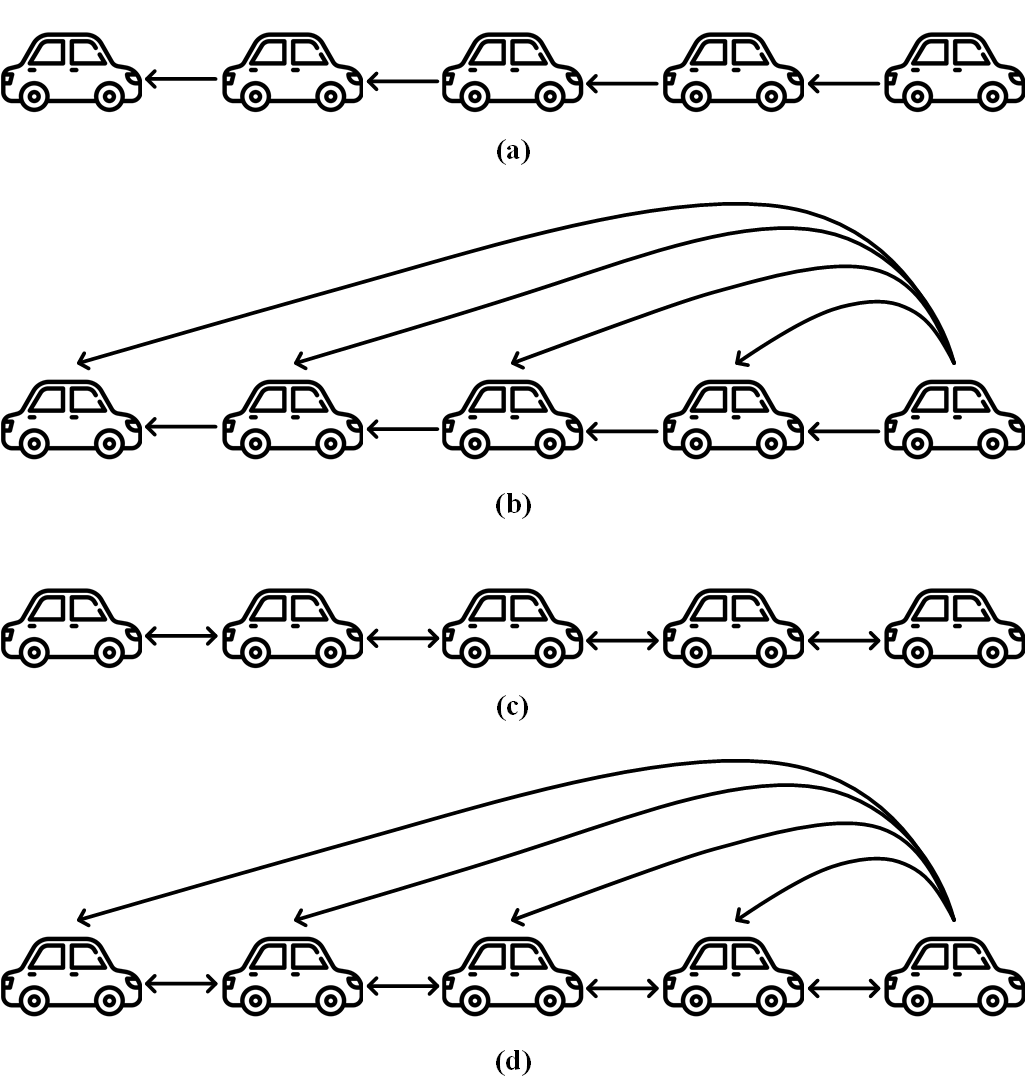
\includegraphics[width=14cm]{figs/fig1.png}
  \caption{~The schematic of the CAV platoon with typical IFTs: (a) Predecessor-Follower (PF); (b) Predecessor-Leader-Follower (PLF); (c) Bi-Directional (BD); and (d) Bi-Directional-Leader (BDL).}
  \label{fig1}
\end{figure}

Consider a group of $n$ CAVs moving along a single lane and forming a CAV platoon where the intra-vehicle communication functions according to the IFT. Fig.~\ref{fig1} shows the schematic of the CAV platoon with typical four IFTs: Predecessor-Follower (PF), (b) Predecessor-Leader-Follower (PLF), (c) Bi-Directional (BD), and (d) Bi-Directional-Leader (BDL). Via intra-vehicle communication (e.g., C-V2X according to the meeting report from Federal Communications Commission \citep{popeo2020federal}), all vehicles share their state information (e.g., the absolute position, the velocity, and the acceleration) with their neighbors according to the IFT. It is assumed that each CAV is equipped with i) an on-board radar responsible for collision detection via measuring the gap distance between any two consecutive vehicles, ii) a built-in GPS sensor for measuring the longitudinal position, iii) a wireless on-board unit for communicating potentially useful information with its proximal vehicles via the C-V2X communication \citep{VerizonNorth2020}, iv) an upper-level controller for calculating the desired longitudinal acceleration based on the parameters obtained, and v) a lower-level controller for determining the throttle and brake actuator inputs so as to track the desired acceleration. Such an assumption is reasonable because the sensing, communication, and actuation units required above are available in modern CAVs and therefore do not require specific changes to the existing vehicle configuration. Note that the information of the surrounding obtained by on-board radar only function as the validation data in case of communication unavailability or failure, as more accurate information can be more efficiently obtained through communication.

\subsection{Vehicle longitudinal dynamic Modeling}
\label{Section 3.1}

A vehicle longitudinal dynamic model mainly consists of the engine, throttle and brake actuators, drive train, transmission, and torque converter. According to Newton's second law, the longitudinal dynamics of vehicle $i$ considering a variety of resistance forces can be modeled by the following equation:

\begin{equation}
  m_ia_i(t)=f_i^e(t)-f_i^g(t)-f_i^w(t)-f_i^r(t)
  \label{eq1}
\end{equation}
where $m_i$ stands for the unknown mass of vehicle $i$; $f_i^e(t)$ is the desired engine force acting on vehicle $i$; $f_i^g(t)$, $\ f_i^w(t)$, and $f_i^r(t)$ denote the gravity component parallel to the road surface, air resistance force, and rolling resistance force, respectively.

The nonlinearity of the system~(\ref{eq1}) is not conducive to controller design. Therefore, a feedback control input in Appendix A is employed to convert it into a linear form:
\begin{equation}
  \tau_i\dot{a_i}\left(t\right)+a_i\left(t\right)=u_i(t)
  \label{eq2}
\end{equation}
where $u_i(t)$ denotes the control input of the lower-level controller, which can be interpreted as the desired acceleration of vehicle $i$, $\tau_i$ is the time constant representing the engine actuator delay.

Reformulate Equation~(\ref{eq2}), the state space equation can be represented as:
\begin{equation}
  {\dot x_i}\left( t \right) = A{x_i}\left( t \right) + B{u_i}\left( t \right)
  \label{eq3}
\end{equation}
with $A = \left[ {\begin{array}{*{20}{c}}
          0 & 1 & 0                          \\
          0 & 0 & 1                          \\
          0 & 0 & { - \frac{1}{{{\tau _i}}}}
        \end{array}} \right]$ and $B = \left[ {\begin{array}{*{20}{c}}
          0 \\
          0 \\
          {\frac{1}{{{\tau _i}}}}
        \end{array}} \right]$,\\
where ${x_i}\left( t \right) = {\left[ {\begin{array}{*{20}{c}}
          {{p_i}\left( t \right)} & {{v_i}\left( t \right)} & {{a_i}\left( t \right)}
        \end{array}} \right]^T} \in {\mathbb{R}^3}$ denotes the state vector of vehicle $i$.

Subject to limited communication, the input for vehicle $i$ are controlled by an appropriate decentralized coupling protocol of communication information:
\begin{equation}
  {u_i} = {u_i}\underbrace {\left( {{x_1}\left( {t - h(t)} \right), \cdots ,{x_i}\left( t \right), \cdots ,{x_n}\left( {t - h(t)} \right)} \right)}_n
  \label{eq4}
\end{equation}
where $ h(t) $ represents the communication delay within the transmission range which assumed to be time-varying according to the variation of the surrounding environment \citep{jia_enhanced_2016,Vukadinovic2018,Vu2020,Martin-Sacristan2020,Pirani2022}. And it satisfies the following constraints:
\begin{equation}
  h(t) \in \left[ {{h_m},{h_M}} \right],\quad \dot h(t) \in \left[ {{d_m},{d_M}} \right],\quad \forall t \geqslant 0
  \label{eq5}
\end{equation}
where $ 0 \leqslant {h_m} \leqslant {h_M} $ and $ {d_m} \leqslant {d_M} \leqslant 1 $.

Here we assume that CAVs adopt the Constant Time Headway (CTH) policy in which CAVs maintain a desired time headway from the reference vehicle. Then the cooperative tracking problem of vehicle $i$ can be formulated as:
\begin{equation}
  \left\{ \begin{gathered}
    \mathop {\lim }\limits_{t \to \infty } \left\| {\sum\limits_{j = 1}^n {\left| {{p_i}(t) - {p_j}(t - h(t)){\text{ + }}{h_{ij}}{v_i}(t)} \right|} } \right\| = 0 \hfill \\
    \mathop {\lim }\limits_{t \to \infty } \left\| {\sum\limits_{j = 1}^n {\left| {{v_i}(t) - {v_j}(t - h(t))} \right|} } \right\| = 0 \hfill \\
    \mathop {\lim }\limits_{t \to \infty } \left\| {\sum\limits_{j = 1}^n {\left| {{a_i}(t) - {a_j}(t - h(t))} \right|} } \right\| = 0 \hfill \\
  \end{gathered}  \right.\forall i = 1, \ldots ,N
  \label{eq6}
\end{equation}
where $ {h_{ij}} =  - {h_{ji}} $ stands for the constant time headway between vehicle $i$ and vehicle $j$.

The consensus goal~(\ref{eq6}) can be achieved by using an appropriate distributed control strategy. Therefore, the vehicle $i$ adjusts its dynamics through the following decentralized coupling protocol computed onboard as:
\begin{equation}
  {u_i} =  - \sum\limits_{j = 1}^n {{a_{ij}}{k_{ij}}^T{{\left[ {\begin{array}{*{20}{c}}
              {{p_i}\left( t \right) - {p_j}\left( {t - h(t)} \right) + {h_{ij}}{v_i}\left( t \right)} & {{v_i}\left( t \right) - {v_j}\left( {t - h(t)} \right)} & {{a_i}\left( t \right) - {a_j}\left( {t - h(t)} \right)}
            \end{array}} \right]}^T}}
  \label{eq7}
\end{equation}
where $ {a_{ij}} $ denotes the weight of edge $ \left( {i,j} \right) $ and $ {a_{ij}} = 0 $ if there is no edge $ \left( {i,j} \right) $; $ {k_{ij}} = {\left[ {\begin{array}{*{20}{c}}
          {{\alpha _{ij}}} & {{\beta _{ij}}} & {{\gamma _{ij}}}
        \end{array}} \right]^T} \in {\mathbb{R}^{3 \times 1}} $ presents the feedback control gain vector, with $ {\alpha _{ij}} $, $ {\beta _{ij}} $, and $ {\gamma _{ij}} $ denoting the control gain of spacing error, speed error, and acceleration error, respectively.






\subsection{CAV platoon Modeling}
\label{Section 3.2}

To prove the consensus of systems~(\ref{eq3}) and~(\ref{eq4}) under the action of coupling protocol~(\ref{eq7}), then the decentralized coupling protocol~(\ref{eq7}) can be reformulated as:
\begin{equation}
  {u_i} =  - \sum\limits_{j = 1}^n {{a_{ij}}{k_{ij}}^T\left[ {{\psi _{ij}}{x_i}(t) - {x_j}(t - h(t))} \right]}
  \label{eq10}
\end{equation}
where $ {\psi _{ij}}{\text{ = }}\left[ {\begin{array}{*{20}{c}}
          1  & {{h_{ij}}} & {} \\
          {} & 1          & {} \\
          {} & {}         & 1
        \end{array}} \right] $ denotes the relationship between the states based on the CTH policy.

Therefore, the dynamics of the error system can be presented as:
\begin{equation}
  \left\{ \begin{gathered}
    {{\dot {\tilde p}}_i} = {{\tilde v}_i} \hfill \\
    {{\dot {\tilde v}}_i} = {{\tilde a}_i} \hfill \\
    {{\dot {\tilde a}}_i} =  - \frac{1}{\tau }{{\tilde a}_i} - \frac{1}{\tau }\sum\limits_{j = 1}^n {{a_{ij}}{k_{ij}}^T\left( {{\psi _{ij}}{x_i}(t) - {x_j}(t - h(t))} \right)}  \hfill \\
  \end{gathered}  \right.
  \label{eq11}
\end{equation}

From Equation~(\ref{eq11}), the dynamics of the closed-loop vehicular network can be recast in a compact form with supermatrices as:
\begin{equation}
  {\dot x_i}\left( t \right) = A{x_i}\left( t \right) - B\sum\limits_{j = 1}^n {{a_{ij}}{k_{ij}}^T\left( {{\psi _{ij}}{x_i}(t) - {x_j}(t - h(t))} \right)}
  \label{eq12}
\end{equation}

\begin{theorem}
  \label{theorem3}
  The CAV platoon under CTH policy with time-varying communication delay can be modeled as a linear time-invariant state time-varying delay system:
  \begin{equation}
    \left\{ \begin{gathered}
      \dot X\left( t \right) = \Psi X\left( t \right) + {\Psi _d}X(t - h(t)),\quad \forall t \geqslant 0 \hfill \\
      X\left( t \right) = \phi \left( t \right),\quad \quad \quad \quad \quad \quad \quad \forall t \in \left[ { - h,0} \right] \hfill \\
    \end{gathered}  \right.
    \label{eq13}
  \end{equation}
  with
  \begin{equation}
    \left\{ {\begin{array}{*{20}{l}}
          {\Psi  = {A^*} - {B^*}\mathcal{F}{E_1} \in {\mathbb{R}^{3n \times 3n}}}                                         \\
          \begin{gathered}
            {\Psi _d} = {B^*}\mathcal{J}{E_2} \in {\mathbb{R}^{3n \times 3n}} \hfill \\
            {A^*} = {I_n} \otimes A \in {\mathbb{R}^{3n \times 3n}} \hfill \\
          \end{gathered}                                                                                      \\
          {{B^*} = {I_n} \otimes B \in {\mathbb{R}^{3n \times n}}}                                                        \\
          \begin{gathered}
            \mathcal{K} = {[{k_{ij}}^T]_{n \times n}} \hfill \\
            \mathcal{H} = \mathcal{A} \circ \mathcal{K} = {[{a_{ij}} \otimes {k_{ij}}^T]_{N \times N}} \in {\mathbb{R}^{n \times 3n}} \hfill \\
            \mathcal{J} = diag\underbrace {\left\{ {{\mathcal{D}_1},{\mathcal{D}_2}, \cdots ,{\mathcal{D}_N}} \right\}}_n \in {\mathbb{R}^{n \times 3{n^2}}} \hfill \\
            {\mathcal{D}_i} = \underbrace {\left[ {{a_{i1}}{k_{i1}}^T,{a_{i2}}{k_{i2}}^T, \cdots ,{a_{in}}{k_{in}}^T} \right]}_n \in {\mathbb{R}^{1 \times 3n}},\forall i \in \mathcal{V} \hfill \\
            \mathcal{F} = diag\underbrace {\left\{ {{\mathcal{H}_1},{\mathcal{H}_2}, \cdots ,{\mathcal{H}_N}} \right\}}_n \in {\mathbb{R}^{n \times 3{n^2}}} \hfill \\
            % {\mathcal{H}_i} = \underbrace {\left[ {{a_{i1}}{k_{i1}}^T{\psi _{i1}},{a_{i2}}{k_{i2}}^T{\psi _{i2}}, \cdots ,{a_{in}}{k_{in}}^T{\psi _{in}}} \right]}_n \in {\mathbb{R}^{1 \times 3n}},\forall i \in \mathcal{V} \hfill \\
            {\mathcal{H}_i} = {\mathcal{D}_i} \circ \underbrace {\left[ {{\psi _{i1}},{\psi _{i2}}, \cdots ,{\psi _{in}}} \right]}_n \in {\mathbb{R}^{1 \times 3n}},\forall i \in \mathcal{V} \hfill \\          
          \end{gathered}                                                                                      \\
          {{E_1} = diag\underbrace {\left\{ {{I_1},{I_1}, \cdots ,{I_1}} \right\}}_n \in {\mathbb{R}^{3{n^2} \times 3n}}} \\
          {{E_2} = {{\underbrace {\left[ {\begin{array}{*{20}{c}}
                            {{I_2}^T} & \cdots & {{I_2}^T}
                          \end{array}} \right]}_n}^T} \in {\mathbb{R}^{3{n^2} \times 3n}}} \\
          {{I_1} = {{\underbrace {\left[ {\begin{array}{*{20}{c}}
                            {{I_3}^T} & \cdots & {{I_3}^T}
                          \end{array}} \right]}_n}^T} \in {\mathbb{R}^{3n \times 3}}}      \\
          {{I_2} = {I_{3n}} \in {\mathbb{R}^{3n \times 3n}}}                                                              \\
          {{I_3} = {I_3} \in {\mathbb{R}^{3 \times 3}}}
        \end{array}} \right.
    \label{eq14}
  \end{equation}
  where $ X\left( t \right) = {\left[ {\begin{array}{*{20}{c}}
            {{x_1}^T} & \cdots & {{x_n}^T}
          \end{array}} \right]^T} \in {\mathbb{R}^{3n}} $ stands for the error state vector of the closed-loop vehicular network; $ \phi  $ is the initial conditions; $ \Psi  $ and $ {\Psi _d} $ are constant matrix according to their definitions.

\end{theorem}


\section{Stability analyses}
\label{Section 4}

In the context of the stability analysis of state delay systems, the Lyapunov-Krasovskii Stability Theorem is a well-known approach extending the second Lyapunov method dedicated to stability analysis \citep{Gu2003}. It includes the "energy" functionals that are positive definite, and decreasing along the trajectories of the system. The Lyapunov-Krasovskii Theorem is stated below:
\begin{lemma}
  \label{lemma3}
  (Lyapunov-Krasovskii Stability Theorem) \citep{Gu2009}. Given system (\ref{eq13}), suppose that $f$ maps $\mathbb{R} \times  $(bounded sets in ${\mathbb{R}^n} \times \mathcal{C} $) into bounded sets in ${\mathbb{R}^n} $, and that $u,v,w:{\mathbb{R}_ + } \to {\mathbb{R}_ + } $ are continuous nondecreasing functions, where additionally $u(s) $ and $v(s) $ are positive for $s > 0 $, and $u(0) = v(0) = 0 $. If there exists a functional $V:\mathbb{R} \times {\mathbb{R}^n} \times \mathcal{C} \to \mathbb{R} $ such that
  \begin{equation}
    \left\{ \begin{gathered}
      u(|\phi \left( 0 \right)|) \leqslant V(t,\phi ) \leqslant v(|\phi {|_h}) \hfill \\
      \dot V(t,\phi ) \leqslant  - w(|\phi \left( 0 \right)|) \hfill \\
    \end{gathered}  \right.
    \label{eq15}
  \end{equation}
  Then the trivial solution of the system (\ref{eq13}) is uniformly stable. If $w(s) > 0 $ for $s > 0 $, then it is uniformly asymptotically stable. If, in addition, $\mathop {\lim }\limits_{s \to \infty } u(s) =  + \infty  $, then it is globally uniformly asymptotically stable. Such a functional $V $ is called a Lyapunov-Krasovskii functional (LKF).
\end{lemma}

The primary idea of Lemma~\ref{lemma3} is to determine a positive definite functional whose derivative with respect to time along the trajectories of the system (\ref{eq13}) is negative definite. In the context of the stability analysis of such systems using LKF, several types of functionals have been provided in the literature. Among them, an integral quadratic term is one of the most relevant components of LKF \citep{pepe_lyapunovkrasovskii_2006}:
\begin{equation}
  V\left( {{X_t}} \right) = \int_{0 - h}^0 {\int_\theta ^0 {{{\dot X}_t}^T(s)R{{\dot X}_t}(s){\text{d}}s\;{\text{d}}\theta } }
  \label{eq16}
\end{equation}
where $ {\dot X_t}(s) = {\dot X}(t + s) $ denotes the state of the state delay system, $ R \succ 0 $ and $ h > 0 $.

The positivity of LKF (\ref{eq16}) is ensured by $ R \succ 0 $. Then another that needs to be clarified is the negation of its derivative. Differentiating this term with respect to the time $t$, we get:
\begin{equation}
  \dot V\left( {{X_t}} \right) = h{\dot X^T}(t)R\dot X(t) - \int_{ - h}^0 {{{\dot X}^T}} (s)R\dot X(s){\text{d}}s
  \label{eq17}
\end{equation}

In order to transform Equation (\ref{eq17}) into a suitable LMI setup, an over-approximate process of the integral terms is adopted since it cannot be straightforwardly converted in the quadratic formulation described above. Therefore, the next problem is to provide a new lower bound of integral quadratic terms of the form:
\begin{equation}
  F(\omega ) = \int_{ - h}^0 {{\omega ^T}} (s)R\omega (s){\text{d}}s
  \label{eq18}
\end{equation}
where $ \omega  $ is a continuous function from $ [a,b] \to {\mathbb{R}^n} $ and consequently integrable.

\begin{corollary}
  \label{coro4}
  Consider a given matrix $ R \succ 0 $. Then, for all continuous function $ \omega  $ in $ [a,b] \to {\mathbb{R}^n} $ the following inequality holds:
  \begin{equation}
    F(\omega ) \geqslant \frac{1}{h}{\left( {\int_{ - h}^0 {\omega (u){\text{d}}u} } \right)^T}R\left( {\int_{ - h}^0 {\omega (u){\text{d}}u} } \right) + \frac{3}{h}{\Omega ^T}R\Omega
    \label{eq19}
  \end{equation}
  where $ \Omega  = \int_{ - h}^0 {\omega (s){\text{d}}s}  - \frac{2}{h}\int_{ - h}^0 {\int_{ - h}^s {\omega (r){\text{d}}r\;{\text{d}}s} }  $.
\end{corollary}

\begin{proof}
  We first construct the function $z$ for all $ u \in [a,b] $ as:
  \begin{equation}
    z(u) = \int_{ - h}^u {\omega (s){\text{d}}s}  - \frac{{u + h}}{h}\int_{ - h}^0 {\omega (s){\text{d}}s}  - \frac{{( - u)(u + h)}}{{{h^2}}}\Theta
    \label{eq20}
  \end{equation}
  where $ \Theta  $ is a constant vector of $ {\mathbb{R}^n} $ to be defined. Moreover, the function $z\left(u\right)$~(\ref{eq20}) satisfies the constrains of Lemma~\ref{lemma1}, that is $ z(0) = z( - h) = 0 $ according to its definition.

  Then, calculating the left-hand-side of the inequality stated in Lemma~\ref{lemma1} leads to:
  \begin{equation}
    \begin{gathered}
      \int_{ - h}^0 {{{\dot z}^T}(u)R\dot z(u){\text{d}}u}  = \int_{ - h}^0 {{\omega ^T}(u)R\omega (u){\text{d}}u}  - \frac{1}{h}{\left( {\int_{ - h}^0 {\omega (u){\text{d}}u} } \right)^T}R\left( {\int_{ - h}^0 {\omega (u){\text{d}}u} } \right) \hfill \\
      \quad \quad \quad \quad \quad \quad \quad  + \int_{ - h}^0 {{{\left( {\frac{{(h + 2u)}}{{{h^2}}}} \right)}^2}{\text{d}}u{\Theta ^T}R\Theta } \; - 2{\Theta ^T}R\int_{ - h}^0 {\left( {\frac{{ - h - 2u}}{{{h^2}}}} \right)\omega (u){\text{d}}u}  \hfill \\
      \quad \quad \quad \quad \quad \quad \quad  + 2\int_{ - h}^0 {\left( {\frac{{( - h - 2u)}}{{{h^2}}}} \right){\text{d}}u} {\Theta ^T}R\left( {\int_{ - h}^0 {\omega (u){\text{d}}u} } \right) \hfill \\
    \end{gathered}
    \label{eq21}
  \end{equation}

  Substituting $ \int_{ - h}^0 { - h - 2u{\text{d}}u}  = 0 $ and applying integration by parts, Equation~(\ref{eq21}) can be simplified as follows:
  \begin{equation}
    \begin{gathered}
      \int_{ - h}^0 {{{\dot z}^T}(u)R\dot z(u){\text{d}}u}  = \int_{ - h}^0 {{\omega ^T}(u)R\omega (u){\text{d}}u}  - \frac{1}{h}{\left( {\int_{ - h}^0 {\omega (u){\text{d}}u} } \right)^T}R\left( {\int_{ - h}^0 {\omega (u){\text{d}}u} } \right) \hfill \\
      \quad \quad \quad \quad \quad \quad \quad \quad  - \frac{3}{{(b - a)}}{\Omega ^T}R\Omega  + \frac{1}{{3(b - a)}}{(\Theta  + 3\Omega )^T}R(\Theta  + 3\Omega ) \hfill \\
    \end{gathered}
    \label{eq22}
  \end{equation}

  Substituting $ \int_{ - h}^0 z (u){\text{d}}u =  - \frac{h}{6}(\Theta  + 3\Omega ) $ and applying Lemma~\ref{lemma1}, it yields:
  \begin{equation}
    \begin{gathered}
      F(\omega ) \geqslant \frac{1}{h}{\left( {\int_{ - h}^0 {\omega (u){\text{d}}u} } \right)^T}R\left( {\int_{ - h}^0 {\omega (u){\text{d}}u} } \right) + h{\Omega ^T}R\Omega  \hfill \\
      \quad \quad \quad \quad \quad \quad \quad \quad  + \frac{{{\pi ^2} - 12}}{{36h}}{(\Theta  + 3\Omega )^T}R(\Theta  + 3\Omega ) \hfill \\
    \end{gathered}
    \label{eq23}
  \end{equation}

  Since $ \frac{{{\pi ^2} - 12}}{{36h}} > 0 $, the third term in the right-hand side of the inequality~(\ref{eq23}) is definite positive independently of the choice of $ \Theta  $. Moreover, the inequality is equivalent to equality if and only if $ \Theta  =  - 3\Omega  $. Furthermore, the definite positiveness of $ F(\omega ) $ is guaranteed by $ R \succ 0 $. This concludes the proof.

\end{proof}



According to Inequality~(\ref{eq17}), another lower bound needed to be determined is the case of $ F(\dot \omega ) $. Therefore, Corollary~\ref{coro4} is rewritten as follows:
\begin{corollary}
  \label{coro5}
  For a given matrix $ R \succ 0 $, the following inequality holds for all continuously differentiable function $ \omega  $ in $ [a,b] \to {\mathbb{R}^n} $:
  \begin{equation}
    \label{eq24}
    F(\dot \omega ) \geqslant {\text{ }}\frac{1}{h}{(\omega (0) - \omega ( - h))^T}R(\omega (0) - \omega ( - h)) + \frac{3}{h}{\tilde \Omega ^T}R\tilde \Omega
  \end{equation}
  where $ \tilde \Omega  = \omega (0) + \omega ( - h) - \frac{2}{h}\int_a^b \omega  (u){\text{d}}u $.
\end{corollary}

Then the following stability theorem is provided.
\begin{theorem}
  \label{theorem6}
  Assume that there exist $ P \in \mathbb{S}_{3n}^ +  $, three matrices $ S,R,Q \in \mathbb{S}_n^ +  $, and $ X \in \mathbb{S}{_{2n}} $ such that the following LMIs are satisfied for $ h = \{ {h_m},{h_M}\}  $ and $ \dot h = \{ {d_m},{d_M}\}  $.

  \begin{equation}
    \label{eq25}
    {\Phi _1}(h,\dot h) = {\Phi _0}(h,\dot h) - \frac{1}{{{h_M}}}{\Gamma ^T}{\Phi _2}\Gamma  \prec 0,
  \end{equation}
  \begin{equation}
    \label{eq26}
    {\Phi _2} = \left[ {\begin{array}{*{20}{c}}
            {\tilde R} & X          \\
            *          & {\tilde R}
          \end{array}} \right] \succ 0
  \end{equation}
  where
  \begin{itemize}
    \item[]
      $ {\Phi _0}(h,\dot h) = \operatorname{He} \left( {G_1^T(h)P{G_0}(\dot h)} \right) + \hat S + \hat Q(\dot h) + {h_M}G_0^T(\dot h)\hat R{G_0}(\dot h) $;                     \\
      $ \Gamma  = {\left[ {\begin{array}{*{20}{c}}
                {K_1^T} & {K_2^T}
              \end{array}} \right]^T} $;\\
      $ {K_1} = \left[ {\begin{array}{*{20}{c}}
                I & { - I} & 0 & 0       & 0 \\
                I & I      & 0 & { - 2I} & 0
              \end{array}} \right] $;\\
      $ {K_2} = \left[ {\begin{array}{*{20}{c}}
                0 & I & { - I} & 0 & 0       \\
                0 & I & I      & 0 & { - 2I}
              \end{array}} \right] $;\\
      $ \hat Q(\dot h) = \operatorname{diag} \left( {Q, - (1 - \dot h)Q,{0_{3n}}} \right) $;\\
      $ \hat S = \operatorname{diag} \left( {S,0, - S,{0_{2n}}} \right) $;\\
      $ \hat R = \operatorname{diag} \left( {R,{0_{3n}}} \right) $;\\
      $ \tilde R = \operatorname{diag} (R,3R) $;\\
      $ {G_0}(\dot h) = \left[ {\begin{array}{*{20}{c}}
                \Psi & {{\Psi _d}}        & 0      & 0 & 0 \\
                I    & { - (1 - \dot h)I} & 0      & 0 & 0 \\
                0    & {(1 - \dot h)I}    & { - I} & 0 & 0
              \end{array}} \right] $;\\
      $ {G_1}(h) = \left[ {\begin{array}{*{20}{c}}
                I & 0 & 0 & 0    & 0                             \\
                0 & 0 & 0 & {hI} & 0                             \\
                0 & 0 & 0 & 0    & {\left( {{h_M} - h} \right)I}
              \end{array}} \right] $.\\
  \end{itemize}
  Then the system (\ref{eq13}) is asymptotically stable for all delay function $h$ satisfying (\ref{eq5}).

\end{theorem}

\begin{proof}
  We first construct the LKF as:
  \begin{equation}
    \label{eq27}
    \begin{gathered}
      V\left( {h,{x_t},{{\dot x}_t}} \right) = {{\tilde x}^T}(t)P\tilde x(t) + \int_{ - h(t)}^0 {{x^T}} (s)Qx(s){\text{d}}s \hfill \\
      \quad \quad \quad \quad \quad  + \int_{ - {h_M}}^0 {{x^T}} (s)Sx(s){\text{d}}s + \int_{ - {h_M}}^0 {\int_\theta ^0 {{{\dot x}^T}(s)R\dot x(s){\text{d}}s\;{\text{d}}\theta } }  \hfill \\
    \end{gathered}
  \end{equation}
  where $ \tilde x(t) = {\left[ {{x^T}(t),\quad \int_{ - h(t)}^0 {{x^T}} (s){\text{d}}s,\quad \int_{ - {h_M}}^{ - h(t)} {{x^T}} (s){\text{d}}s} \right]^T} $.

  The positivity of LKF (\ref{eq27}) is ensured by $ P \succ 0 $, $ Q \succ 0 $, $ S \succ 0 $, and $ R \succ 0 $. Then, the negation of its derivative needs to be clarified. Differentiating the functional (\ref{eq17}) along the trajectories of (\ref{eq13}) leads to:
  \begin{equation}
    \label{eq28}
    \dot V\left( {h,{x_t},{{\dot x}_t}} \right) = \zeta _1^T(t){\Phi _0}(h,\dot h){\zeta _1}(t) - \int_{ - {h_M}}^0 {{{\dot x}^T}} (s)R\dot x(s){\text{d}}s,
  \end{equation}
  where $ {\zeta _1}(t) = \left[ {\begin{array}{*{20}{c}}
            {x(t)}                                              \\
            {x(t - h(t))}                                       \\
            {x\left( {t - {h_M}} \right)}                       \\
            {\frac{1}{{h(t)}}\int_{ - h(t)}^0 x (s){\text{d}}s} \\
            {\frac{1}{{{h_M} - h(t)}}\int_{ - {h_M}}^{ - h(t)} x (s){\text{d}}s}
          \end{array}} \right] $.

  Notice the Equation (\ref{eq28}) can be obtained by substituting $ \tilde x(t) = {G_1}(h){\zeta _1}(t) $ and $ \dot {\tilde x}(t) = {G_0}(\dot h){\zeta _1}(t) $ into the partial differential of Equation (\ref{eq27}).

  Then split the integral interval of Equation (\ref{eq28}) into two parts: $ [ - {h_M}, - h(t)] $ and $ [ - {h_M},0] $, and apply Corollary~\ref{coro5} respectively to get:
  \begin{equation}
    \label{eq29}
    - \int_{t - {h_M}}^t {{{\dot x}^T}} (s)R\dot x(s){\text{d}}s \leqslant  - \zeta _1^T(t)\left( {\frac{1}{{h(t)}}K_1^T\tilde R{K_1}} \right.\left. { + \frac{1}{{{h_M} - h(t)}}K_2^T\tilde R{K_2}} \right){\zeta _1}(t)
  \end{equation}
  According to the constraint of the Lemma~\ref{lemma2}, assume there exists a $X$ so that $ {\Phi _2} \succ 0 $, then the following inequality holds:
  \begin{equation}
    \label{eq30}
    - \int_{t - {h_M}}^t {{{\dot x}^T}} (s)R\dot x(s){\text{d}}s \leqslant  - \frac{1}{{{h_M}}}\zeta _1^T(t){\Gamma ^T}{\Phi _2}\Gamma {\zeta _1}(t),
  \end{equation}

  Substituting Inequality~(\ref{eq30}) into Equation~(\ref{eq28}), it yields:
  \begin{equation}
    \label{eq31}
    \begin{gathered}
      \dot V\left( {h,{x_t},{{\dot x}_t}} \right) \leqslant \zeta _1^T(t){\Phi _0}(h,\dot h){\zeta _1}(t) - \frac{1}{{{h_M}}}\zeta _1^T(t){\Gamma ^T}{\Phi _2}\Gamma {\zeta _1}(t) \hfill \\
      \quad \quad \quad \quad \quad  = \zeta _1^T(t)\left( {{\Phi _0}(h,\dot h) - \frac{1}{{{h_M}}}{\Gamma ^T}{\Phi _2}\Gamma } \right){\zeta _1}(t) \hfill \\
      \quad \quad \quad \quad \quad {\text{ = }}\zeta _1^T(t){\Phi _1}(h,\dot h){\zeta _1}(t) \hfill \\
    \end{gathered}
  \end{equation}

  Equation~(\ref{eq31}) guarantees $ \dot V\left( {h,{x_t},{{\dot x}_t}} \right) $ is negative definite by restraining $ {\Phi _1}(h,\dot h) \prec 0 $. Since the matrix $ {\Phi _1}(h,\dot h) $ is affine, and consequently convex, with respect to $ h(t) $ and $ \dot h(t) $, it is necessary and sufficient to ensure that $ {\Phi _1}(h,\dot h) \prec 0 $ stays at the vertices of the intervals $ \left[ {0,{h_M}} \right] \times \left[ {{d_m},{d_M}} \right] $. In summary, $ \dot V\left( {h,{x_t},{{\dot x}_t}} \right) $ is negative definite if there exists a matrix $X$ such that $ {\Phi _2} \succ 0 $ and if $ {\Phi _1}(h,\dot h) \prec 0 $, for all $ (h,\dot h) \in \left[ {0,{h_M}} \right] \times \left[ {{d_m},{d_M}} \right] $. This concludes the proof.

\end{proof}

\begin{remark}
  \label{remark7}
  The code for constructing the LMIs in Theorem~\ref{theorem6} has been uploaded to GitHub for subsequent research. The corresponding URL is attached in Appendix B.
\end{remark}

\section{Numerical analyses}
\label{Section 5}
In this section, extensive numerical simulations and analyses on tracking performance and safety conditions are conducted to illustrate the main results. Moreover, the tracking performance of homogeneous and heterogeneous CAV platoon is analyzed separately.

\subsection{Numerical Setup}
\label{Section 5.1}
To provide a comprehensive performance evaluation analysis, we consider a CAV platoon consisting of 5 CAVs interconnected by the four IFTs shown in Fig.~\ref{fig1}. The Leader CAV drives under a given speed profile while the other CAVs drive under the control strategy. It is worth clarifying that each CAV in the platoon communicates only with the neighbors set in the IFT. Additionally, the control parameters need to be set according to the specific control strategy in practice. For further analysis, parameters for both network and traffic simulation are set in Table~\ref{table1}, for simplicity but without loss of generality. It should be noted that the weights of the weighted adjacency matrix are set to $ {a_{ij}} = \frac{1}{{{d_i}}},\forall (i,j) \in \mathcal{E} $ in order to denote that the information of each neighbor has an equal impact on the control decision. As for the time-varying delay, the time-varying equation is given below in the form of the Bessel function of the first kind, whose time-varying curve is shown in Fig.~\ref{fig2}, satisfying the constraint in Equation (\ref{eq5}):
\begin{equation}
  \label{eq51}
  {J_{40}}(t) = \sum\limits_{k = 0}^\infty  {\frac{{{{( - 1)}^k}}}{{k!(k + 40)!}}} {\left( {\frac{{t{\text{ + }}30}}{2}} \right)^{2k + 40}},\quad t \geqslant 0.
\end{equation}


\begin{figure}
  \centering

  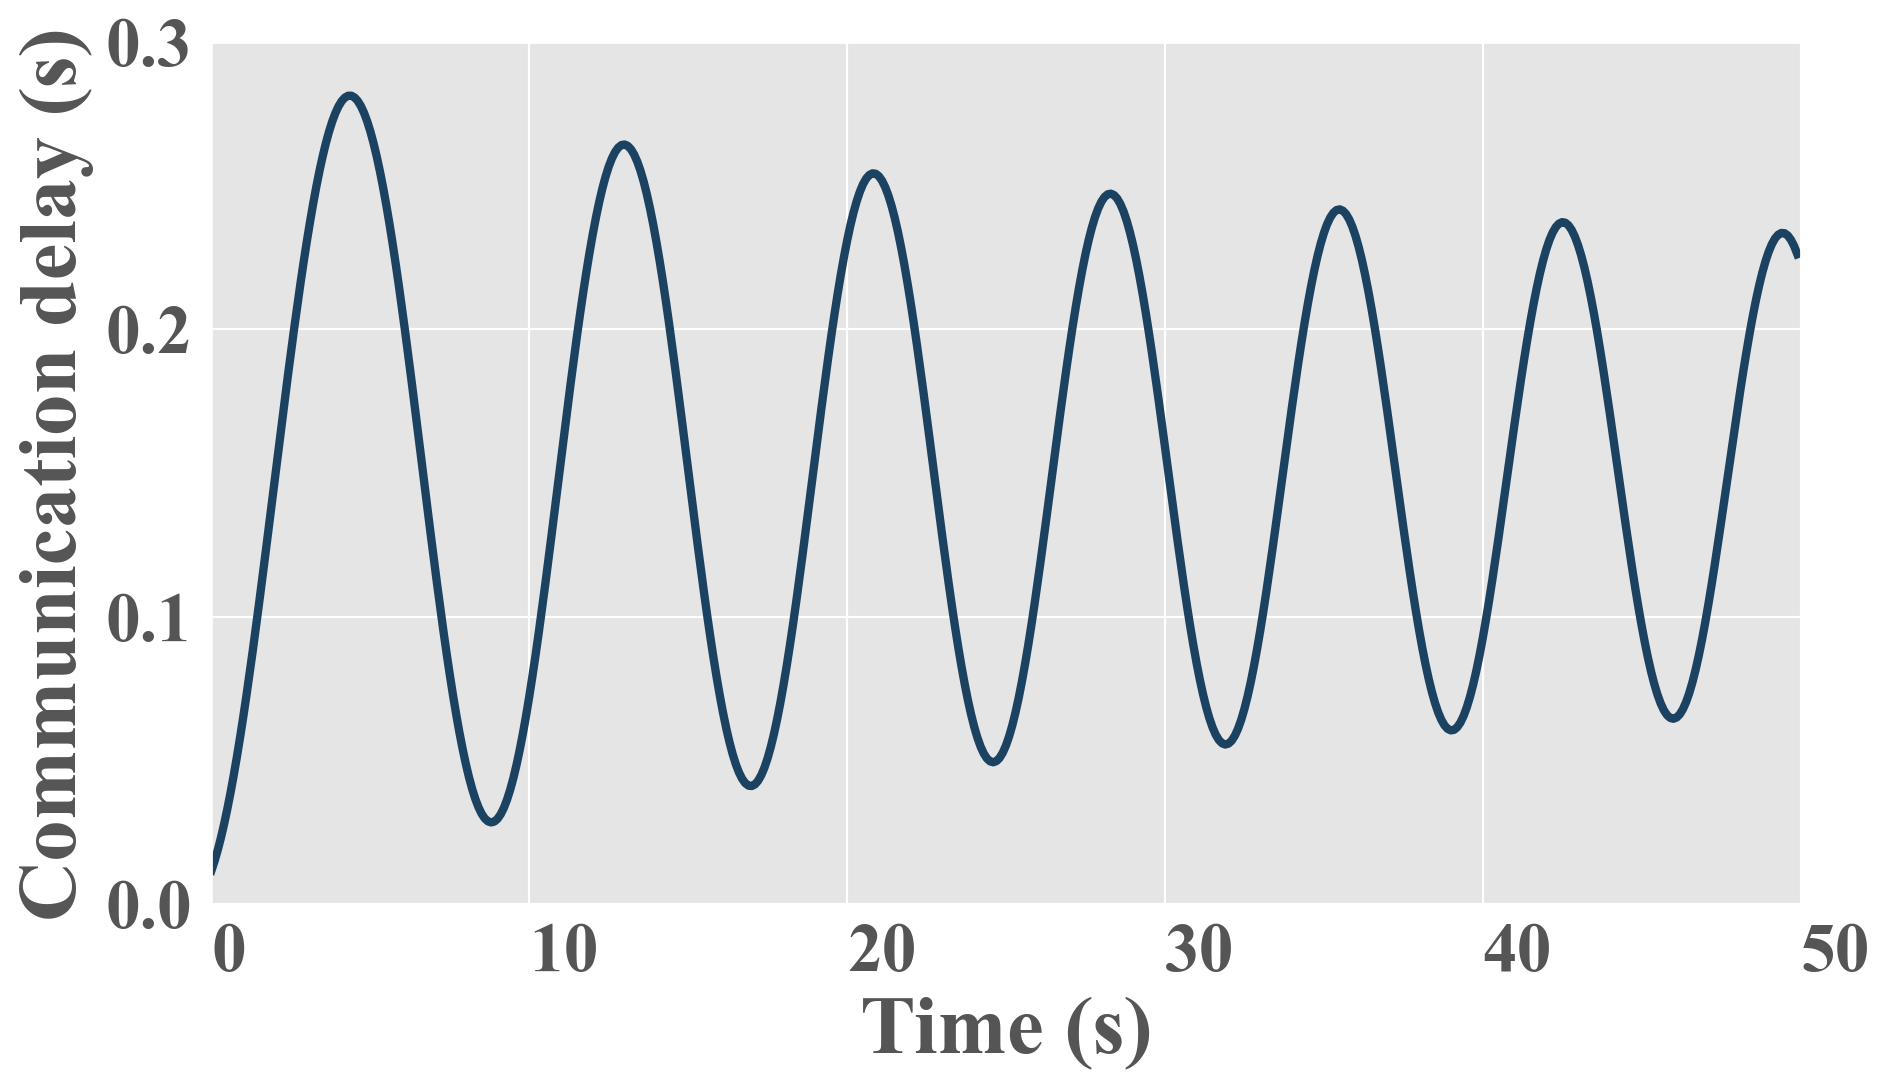
\includegraphics[width=12cm]{figs/fig2.png}
  \caption{~The curve of time-varying communication delay.}
  \label{fig2}
\end{figure}

\begin{table}
  \centering
  \setlength{\abovecaptionskip}{0pt}
  \setlength{\belowcaptionskip}{10pt}%设置标题与表格的距离
  \begin{threeparttable}[b]

    \caption{~Network and traffic simulation parameters.}
    \label{table1}
    {\begin{tabular}{lc} \toprule
        Parameters                                         & Value               \\ \midrule
        Platoon size $n$                                   & 5 vehicles          \\
        Vehicle length $L$                                 & 5 [m]               \\
        Engine actuator delay $\tau_i$                     & 0.2 [s] \tnote{1}   \\
        Weight of edge $\left( {i,j} \right) \quad a_{ij}$ & $\frac{1}{{{d_i}}}$ \\
        Minimum communication delay $h_{m}$                & 0 [m]               \\
        Maximum communication delay $h_{M}$                & 0.3 [m]             \\
        Minimum communication delay slope $d_{m}$          & -0.1                \\
        Maximum communication delay slope $d_{M}$          & 0.1                 \\
        \bottomrule
      \end{tabular}}
    \begin{tablenotes}
      \item[1] \citep{Wang2018a,Zhou2020}
    \end{tablenotes}
  \end{threeparttable}
\end{table}

Moreover, for the sake of evaluating the tracking performance under the four IFTs of the homogeneous and heterogeneous CAV platoon, we adopt two representative leader maneuvers, namely:
\begin{enumerate}
  \item \textbf{Trapezoidal signal}: The leader suddenly decelerates to $14.6m/s$ at $ - 0.15m/{s^2}$ and keeps it for $36s$. Then the leader accelerates back to $20m/s$ at $ 0.3m/{s^2} $(see Fig.~\ref{fig3}(a, b)).
  \item \textbf{Oscillation signal}: The leader suddenly accelerates to $23.6m/s$ in $12s$ and keeps the velocity for $15s$. Then the leader decelerates to $16.4m/s$ in $12s$ and accelerates back to $20m/s$ in $12s$ (see Fig.~\ref{fig3}(c, d)).
\end{enumerate}

\begin{figure}

  \centering
  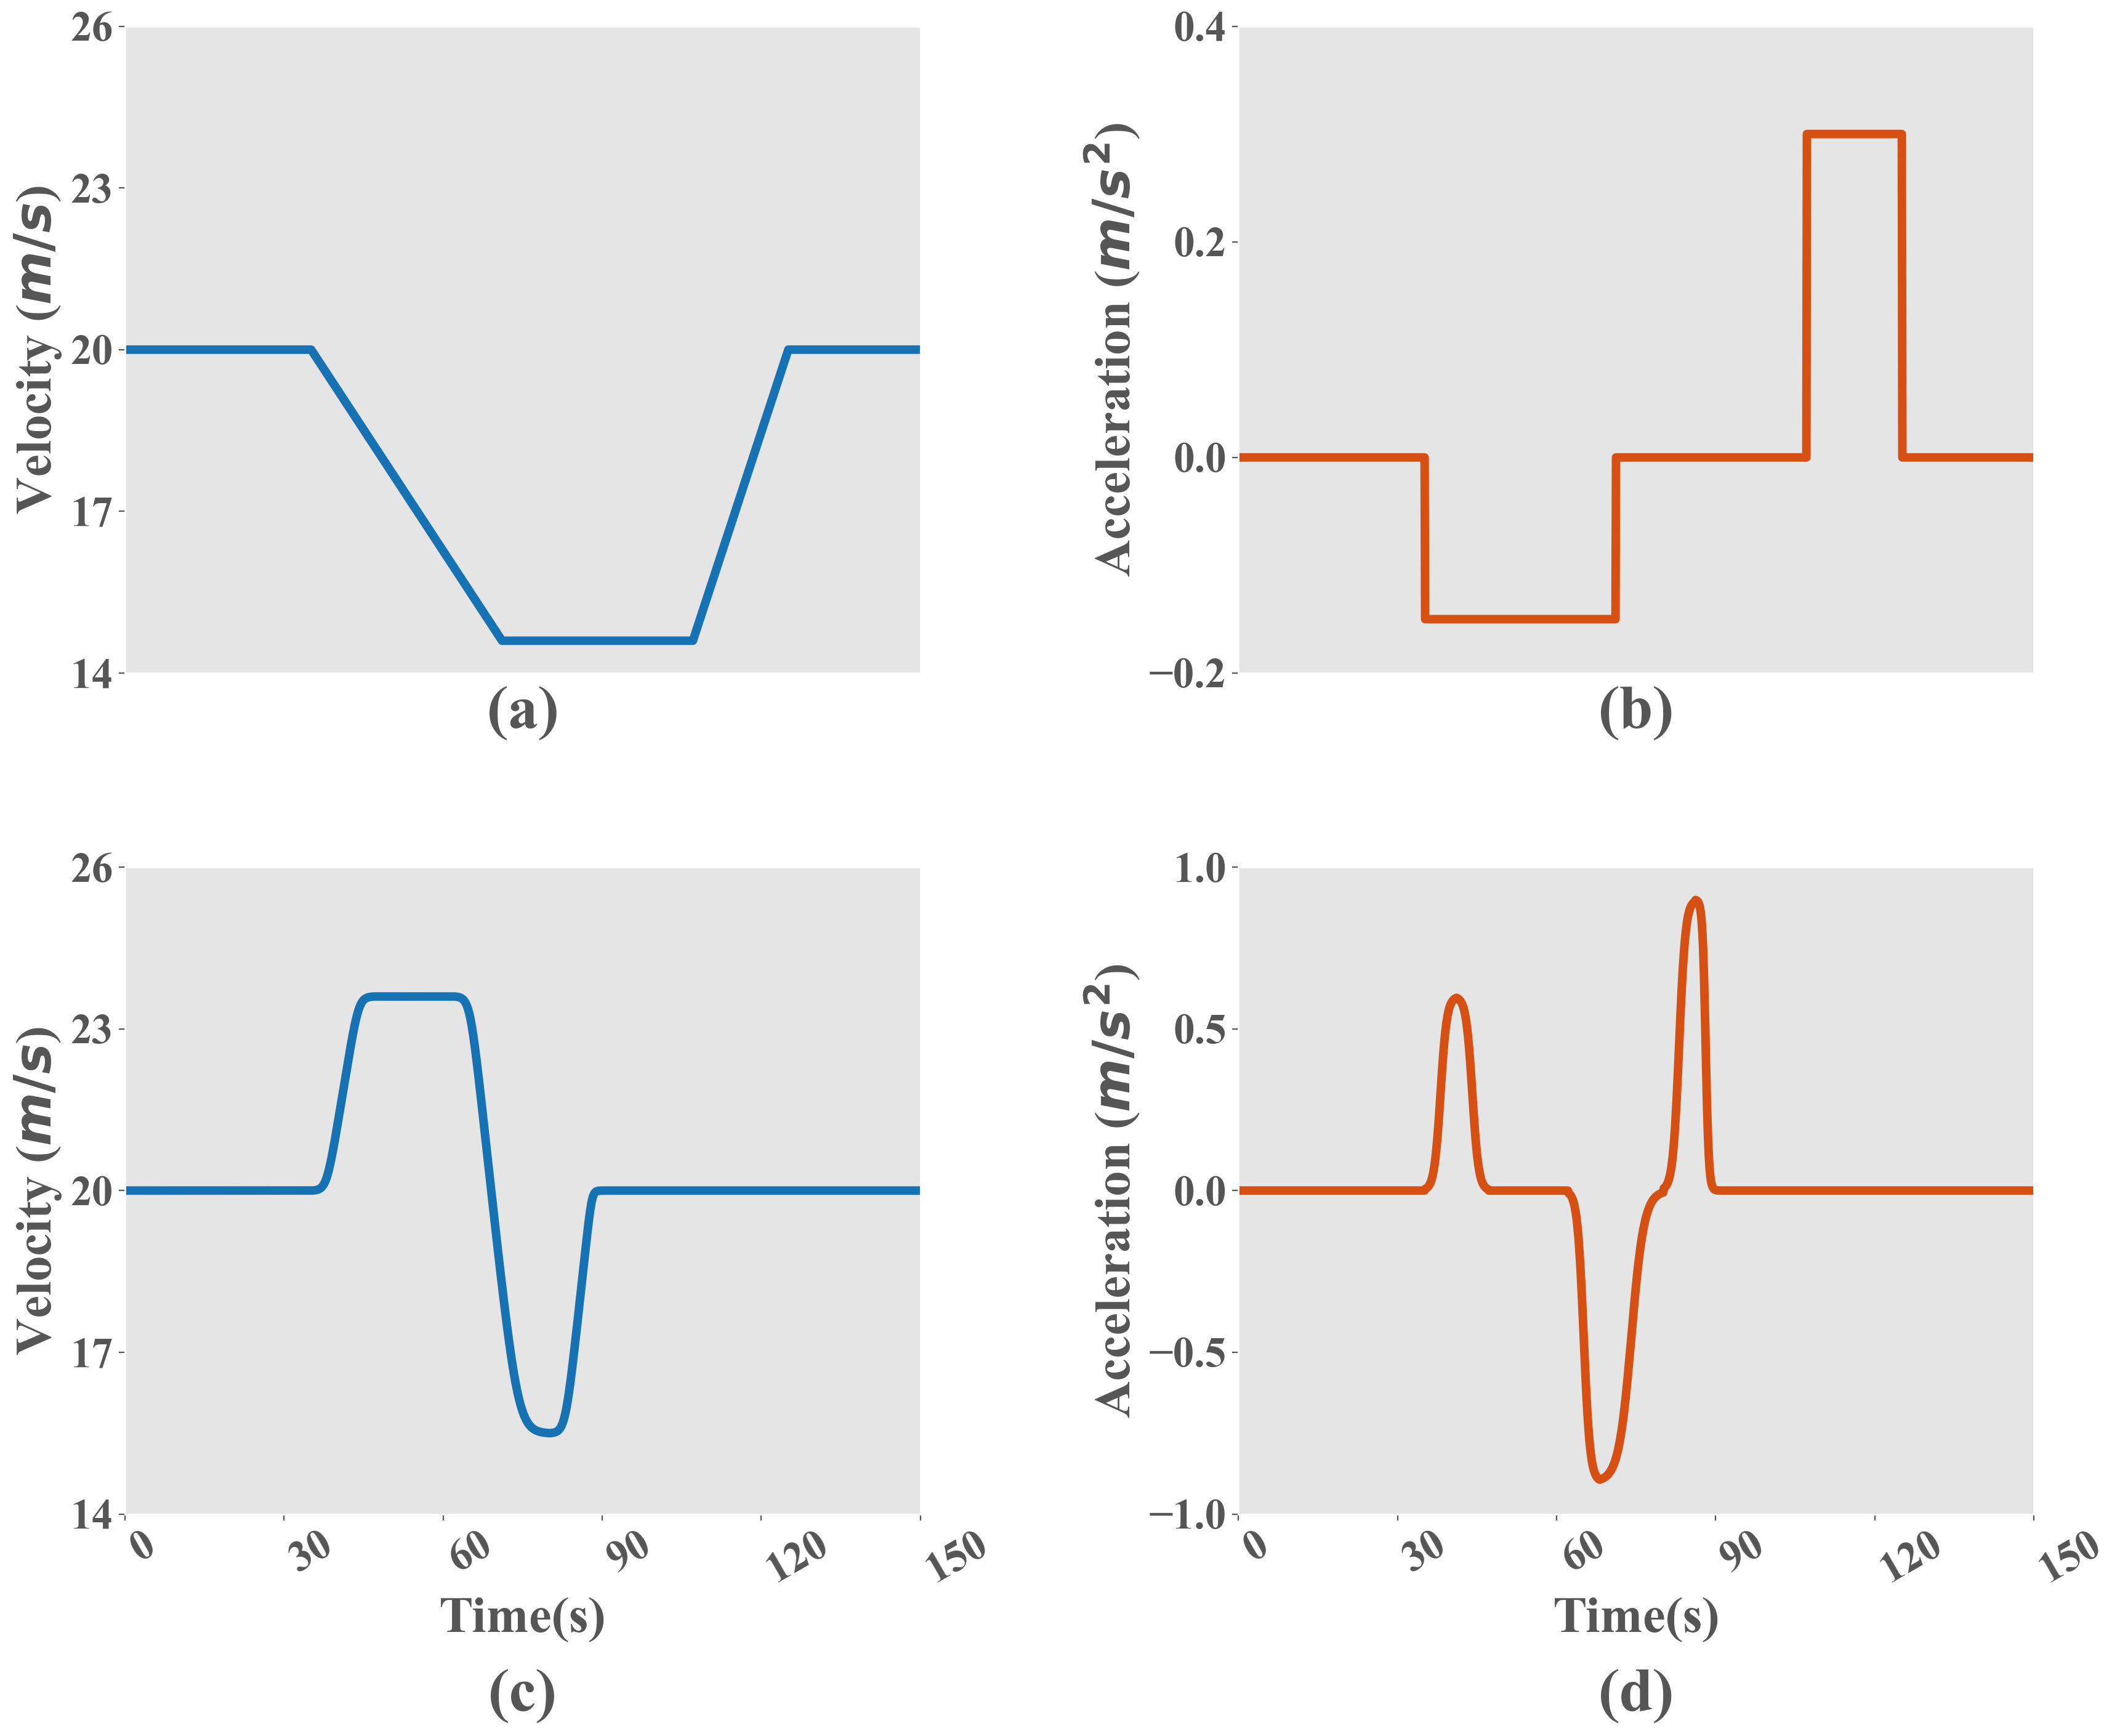
\includegraphics[width=14cm]{figs/fig3.png}
  \caption{~The two representative leader maneuvers: (a) and (b) denotes the velocity and acceleration of the trapezoidal signal, respectively; (c) and (d) denote the velocity and acceleration of the oscillation signal, respectively.}
  \label{fig3}

\end{figure}


\subsection{Numerical analyses of the homogeneous CAV platoon}
\label{Section 5.2}
In this subsection, the homogeneous CAV platoon is taken as the object of analysis, where each CAV in the platoon takes the same control parameters that meet the Theorem~\ref{theorem6}: $ {k_i} = {[0.3,0.3,0.2]^T} $ and $ {h_i} = 0.6 $. Corresponding matrixes $ P,S,Q,R, $ and $X$ can be found in Appendix B. Moreover, a detailed analysis is carried out on the tracking performance and safety conditions.

\subsubsection{Tracking performance analyses}
\label{Section 5.2.1}
After the CAV platoon is formed and each CAV reaches the equilibrium state where the tracking error is zero, we apply the trapezoidal signal shown in Fig.~\ref{fig3}(a,b) as the leader maneuver to evaluate the tracking performance of the four IFTs under investigation. The corresponding results are presented in Fig.~\ref{fig4}, which shows how the different CAVs in the CAV platoon track the leader motion under the trapezoidal signal. As expected in the theoretical results, all CAVs are capable of tracking the leader motion smoothly with a steady-state error of 0. Transient variations in leader motion can cause abrupt changes in tracking error, which disappear over time thanks to stability. An additional conclusion can be drawn that IFTs receiving information from the leader maintain a smoother tracking process without causing overshoot despite amplifying the tracking error compared to IFTs that do not. Furthermore, the adoption of bidirectional communication significantly reduces the magnitude of the error amplification along the CAV platoon, which in turn contributes to the maintenance of string stability.

\begin{figure}

  \centering
  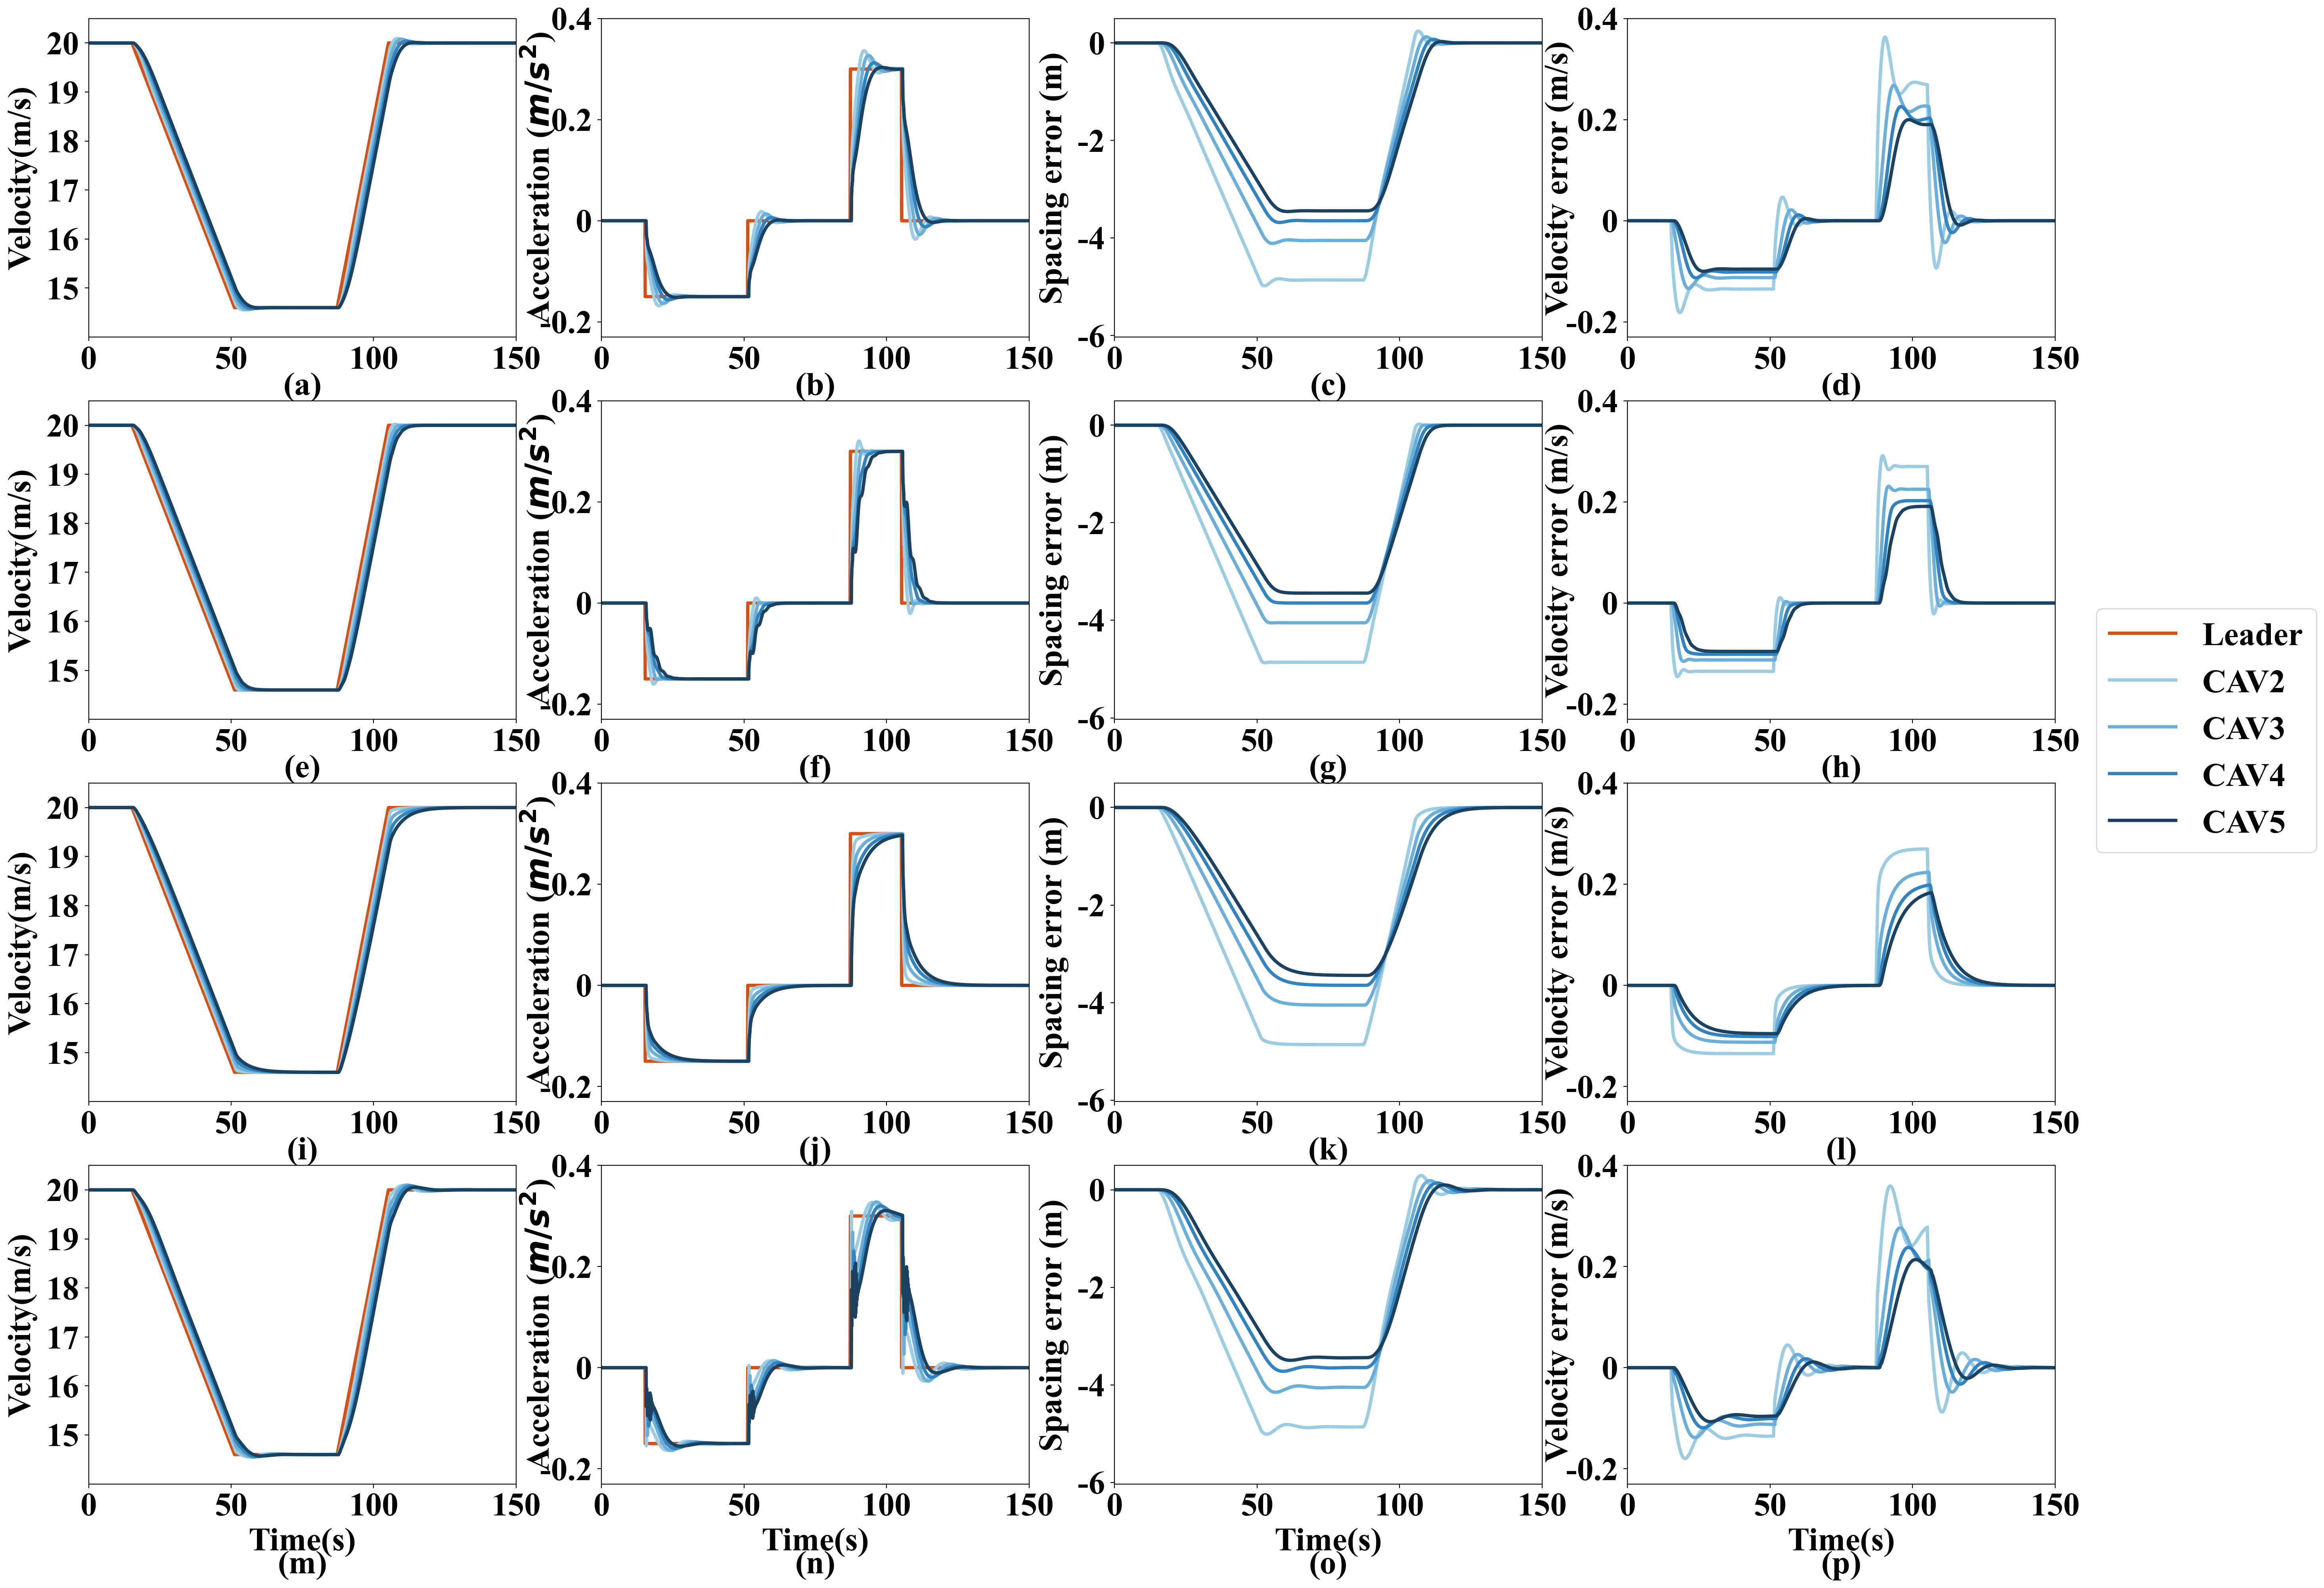
\includegraphics[width=14cm]{figs/fig4.png}
  \caption{~Tracking performance of the homogeneous CAV platoon for the Trapezoidal signal in Fig. 3(a,b) under the four IFTs: (a), (b), (c), and (d) present tracking results under PF, including the velocity, tracking error of position, tracking error of velocity, and tracking error of acceleration, respectively; (e), (f), (g), and (h) show the case under PLF; (i), (j), (k), and (l) denote the case under BD; (m), (n), (o), and (p) show the case under BDL.}
  \label{fig4}
\end{figure}

\begin{figure}

  \centering
  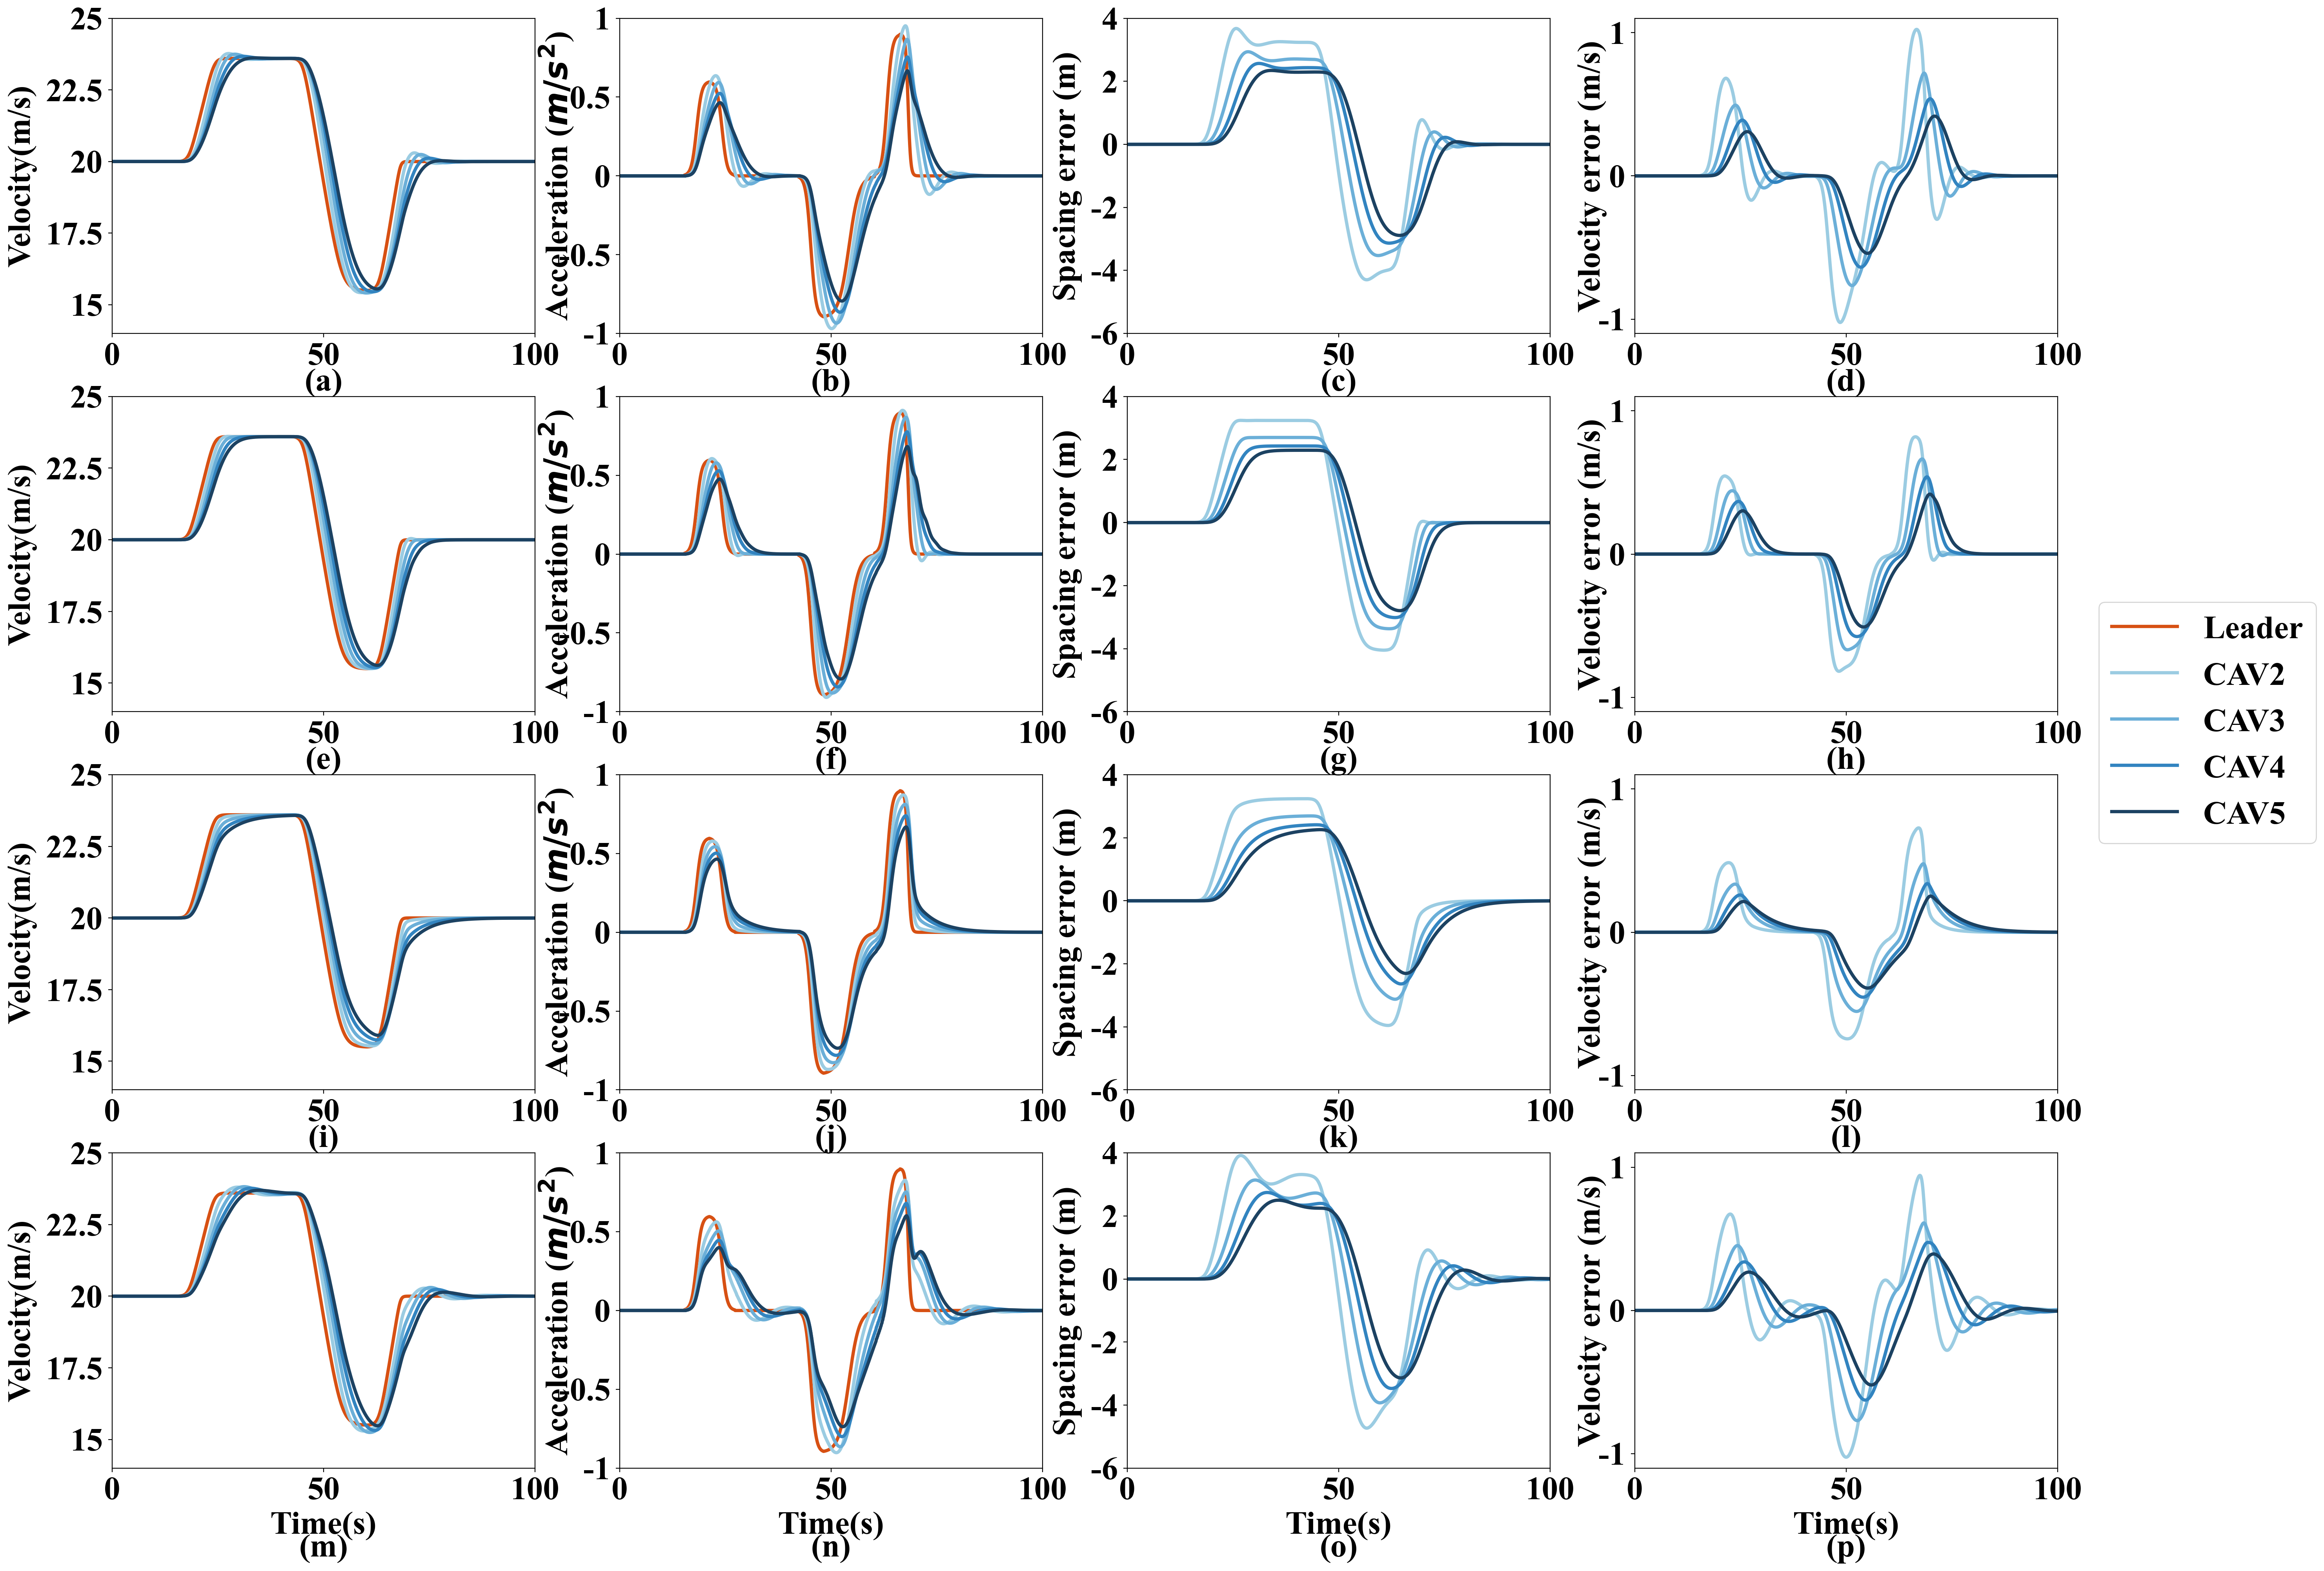
\includegraphics[width=14cm]{figs/fig5.png}
  \caption{~Tracking performance of the homogeneous CAV platoon for the Oscillation signal in Fig. 3(c,d) under the four IFTs: (a), (b), (c), and (d) present tracking results under PF, including the velocity, tracking error of position, tracking error of velocity, and tracking error of acceleration, respectively; (e), (f), (g), and (h) show the case under PLF; (i), (j), (k), and (l) denote the case under BD; (m), (n), (o), and (p) show the case under BDL.}
  \label{fig5}
\end{figure}

Furthermore, the tracking performance of the four IFTs has also been adopted here for the oscillation signal defined in Fig.~\ref{fig3}(c, d). The corresponding tracking performance of the four IFTs is illustrated in Fig.~\ref{fig5}. Under the oscillation signal, the four IFTs still maintain excellent tracking performance as shown in Fig.~\ref{fig5} where each vehicle adjusts to changes in leader motion and returns to the equilibrium state with zero steady-state error. Besides, the similar phenomenon and conclusion as in Fig.~\ref{fig4} can be obtained that maintaining communication with the Leader and using bi-directional communication improves the tracking performance.

Moreover, parallel to the stability studied by tracking performance, we selected two widely accepted indicators for evaluating transient response: Setting time (ST) and Number of oscillations (NOO) for further investigation of the transient response performance of different IFTs. ST refers to "the time required for the response curve to reach and stay within a range of certain percentage (2\%) of the final value". While NOO refers to "the number of deviations of the response curve from the final value caused by errors in the setting time". Of these two indicators, ST describes the time for the controller to recover from transient response to equilibrium, that is, the speed in the fundamental objective, while NOO is concerned with another fundamental objective, accuracy. Note that the NOO rather than the more general indicator, maximum overshoot, is chosen here to signify accuracy because the two leader-based IFTs of the four IFTs do not produce overshoot within setting time. Moreover, a smaller NOO means less acceleration and deceleration changes, which represents a more comfortable driving experience. Also, since the investigation is on the differences in the transient response of different IFTs, the form of the leader motion has little effect on this, so the results are analyzed here only for the case under Trapezoidal signal.

\begin{figure}

  \centering
  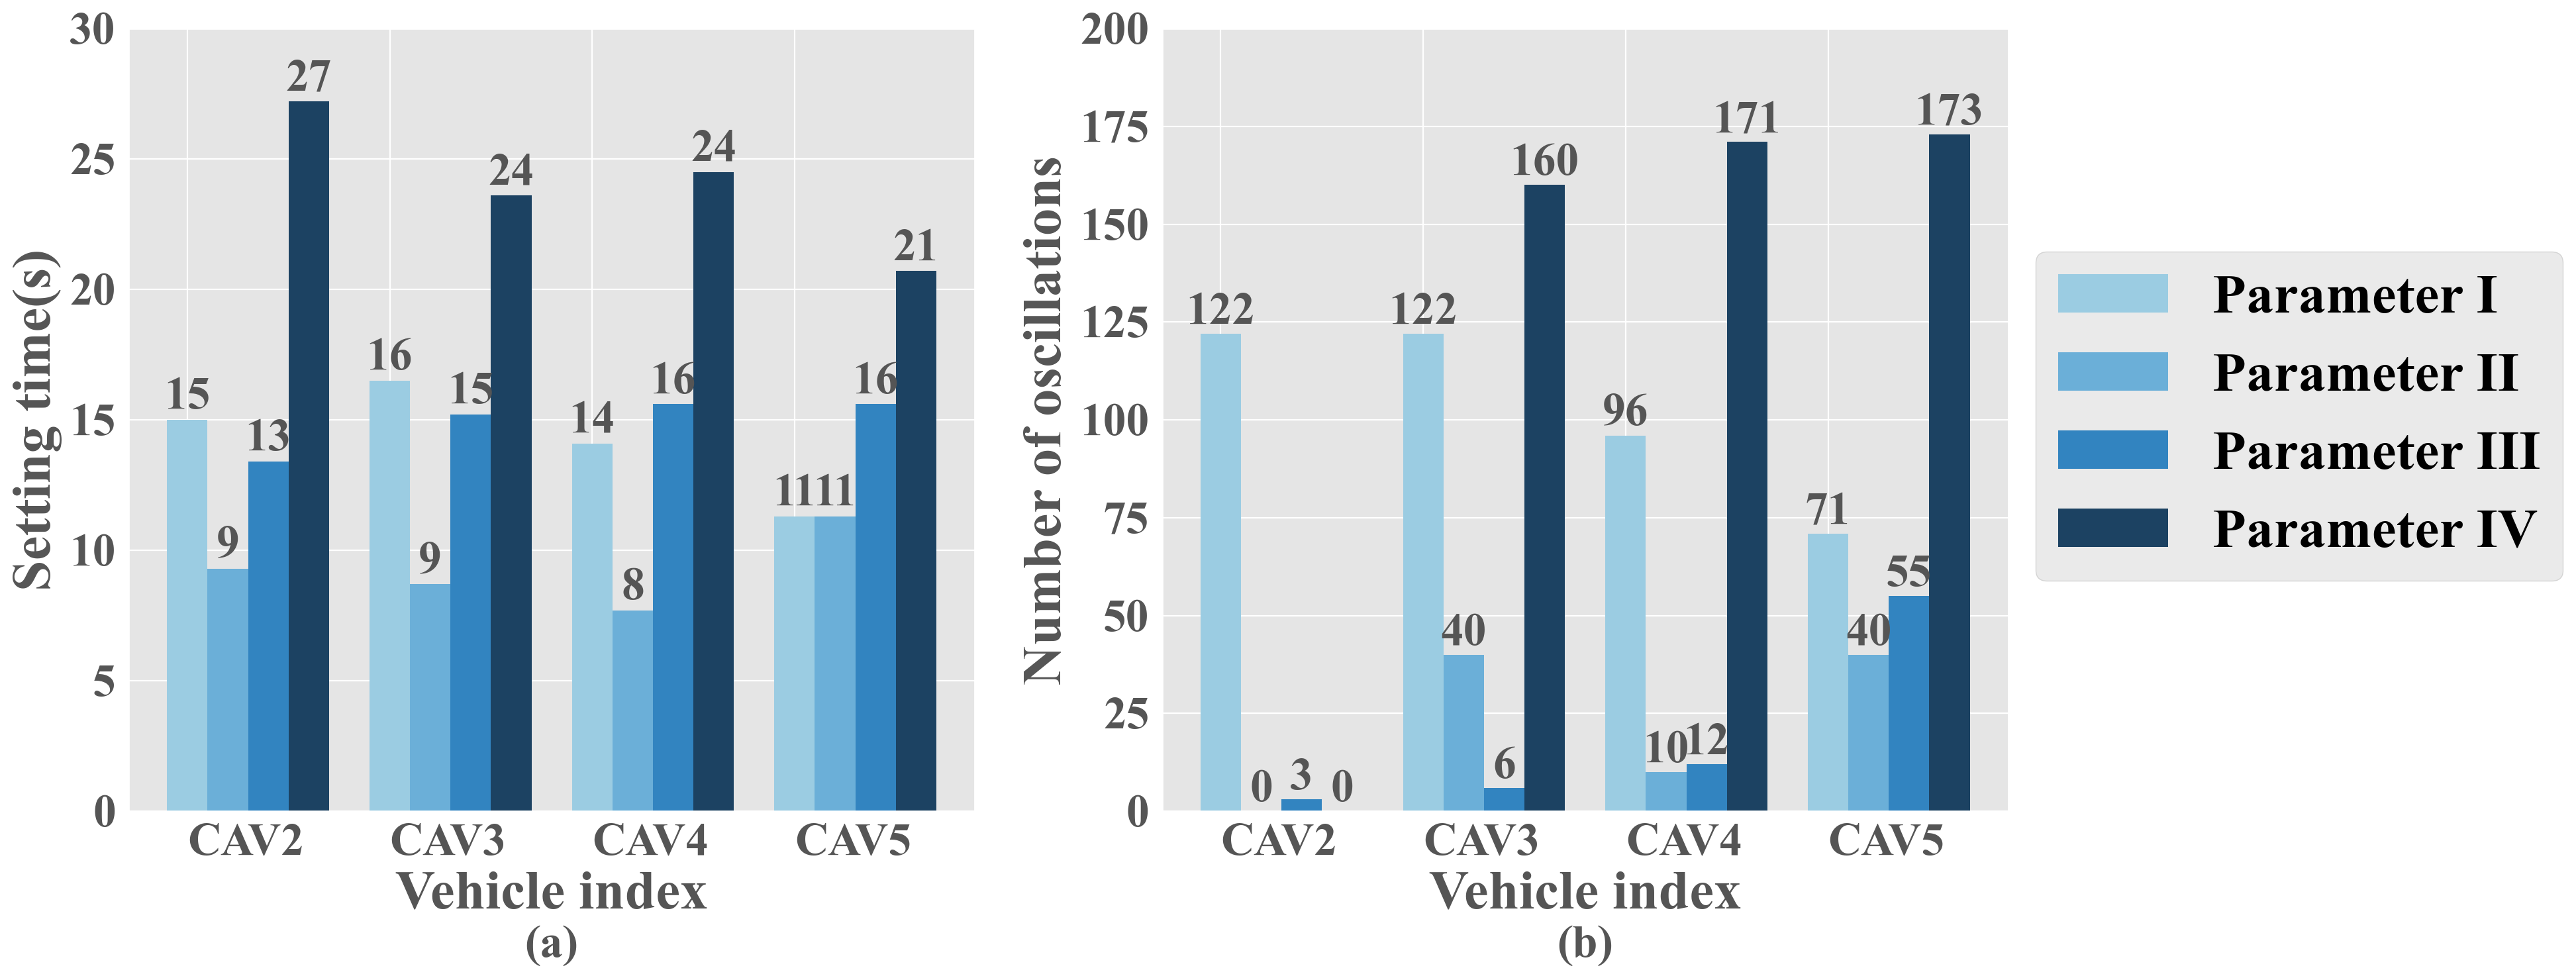
\includegraphics[width=14cm]{figs/fig6.png}
  \caption{~Indicators for evaluating the transient response of each CAV among the CAV platoon under the four IFTs: (a) the case of setting time; (b) the case of number of oscillations.}
  \label{fig6}
\end{figure}

Fig.~\ref{fig6} compares different IFTs on the two indicators of transient response. One conclusion that can be obtained is that the additional communication with the Leader significantly reduces ST and NOO which means it helps to achieve faster and more accurate control, as shown previously in the tracking performance. Moreover, with vehicle index increasing, both ST and NOO increase under each IFT. However, for Leader-based IFTs (PLF and BDL), the magnitude of this increase is less significant than that of PF and BD. Besides, the ST of CAV2 under PF is only 57\% of the one under BD, but the ST of CAV5 under PF is 108\% of the one under BD. Although PF can maintain relatively good tracking when the length of the CAV platoon is short, BD is more suitable as an IFT for CAV platoon with longer length. This phenomenon also indicates that bi-directional communication can effectively balance the tracking performance among the CAV platoon. Furthermore, the Leader-based IFTs eliminate the overshoot resulting in NOO=0 by communicating with the Leader. For PF and BD, the conclusion on NOO is similar to the one drawn on ST. Therefore, the corresponding analysis is omitted.


\subsubsection{Safety analyses considering hard braking maneuver}
\label{Section 5.2.2}

To further evaluate the safety in all the different driving and communication scenarios, we have also quantitatively analyzed the possible emergence of critical driving situations for all IFTs under investigation by exploiting the safety indicator Deceleration Rate to Avoid the Crash (DRAC), which is well known in the literature \citep{fu2021comparison,fu2021random}. This indicator presents the deceleration rate needed to be applied by a vehicle to avoid a collision with another vehicle which can be defined for each vehicle $i$ at the time $t$ as follows:
\begin{equation}
  DRA{C_i}(t) = \frac{{{{\left( {{v_i}(t) - {v_{i - 1}}(t)} \right)}^2}}}{{2\left( {{p_{i - 1}}(t) - {p_i}(t) - L} \right)}}
  \label{eq522}
\end{equation}

Moreover, we consider hard braking maneuver as an additional scenario for evaluation, where the Leader decelerates from $20m/s$ to $0m/s$ within $20s$. Fig.~\ref{fig7} displays how the CAV platoon reacts to hard braking scenario for the four IFTs under investigation. Similarly, CAVs in the CAV platoon under each IFTs tracks the Leader motion accurately and decelerates to $0m/s$ without collision. Furthermore, the DRAC of different CAVs under different IFTs in hard braking maneuver is presented as box plots in Fig.~\ref{fig8}. It is worth mentioning that the DRAC of the Leader is omitted since it has no predecessor, which will raise the risk of collisions. Besides, the CAV2, CAV3, CAV4, and CAV5 refer to the second, third, fourth, and fifth CAV in the CAV platoon, respectively.

\begin{figure}

  \centering
  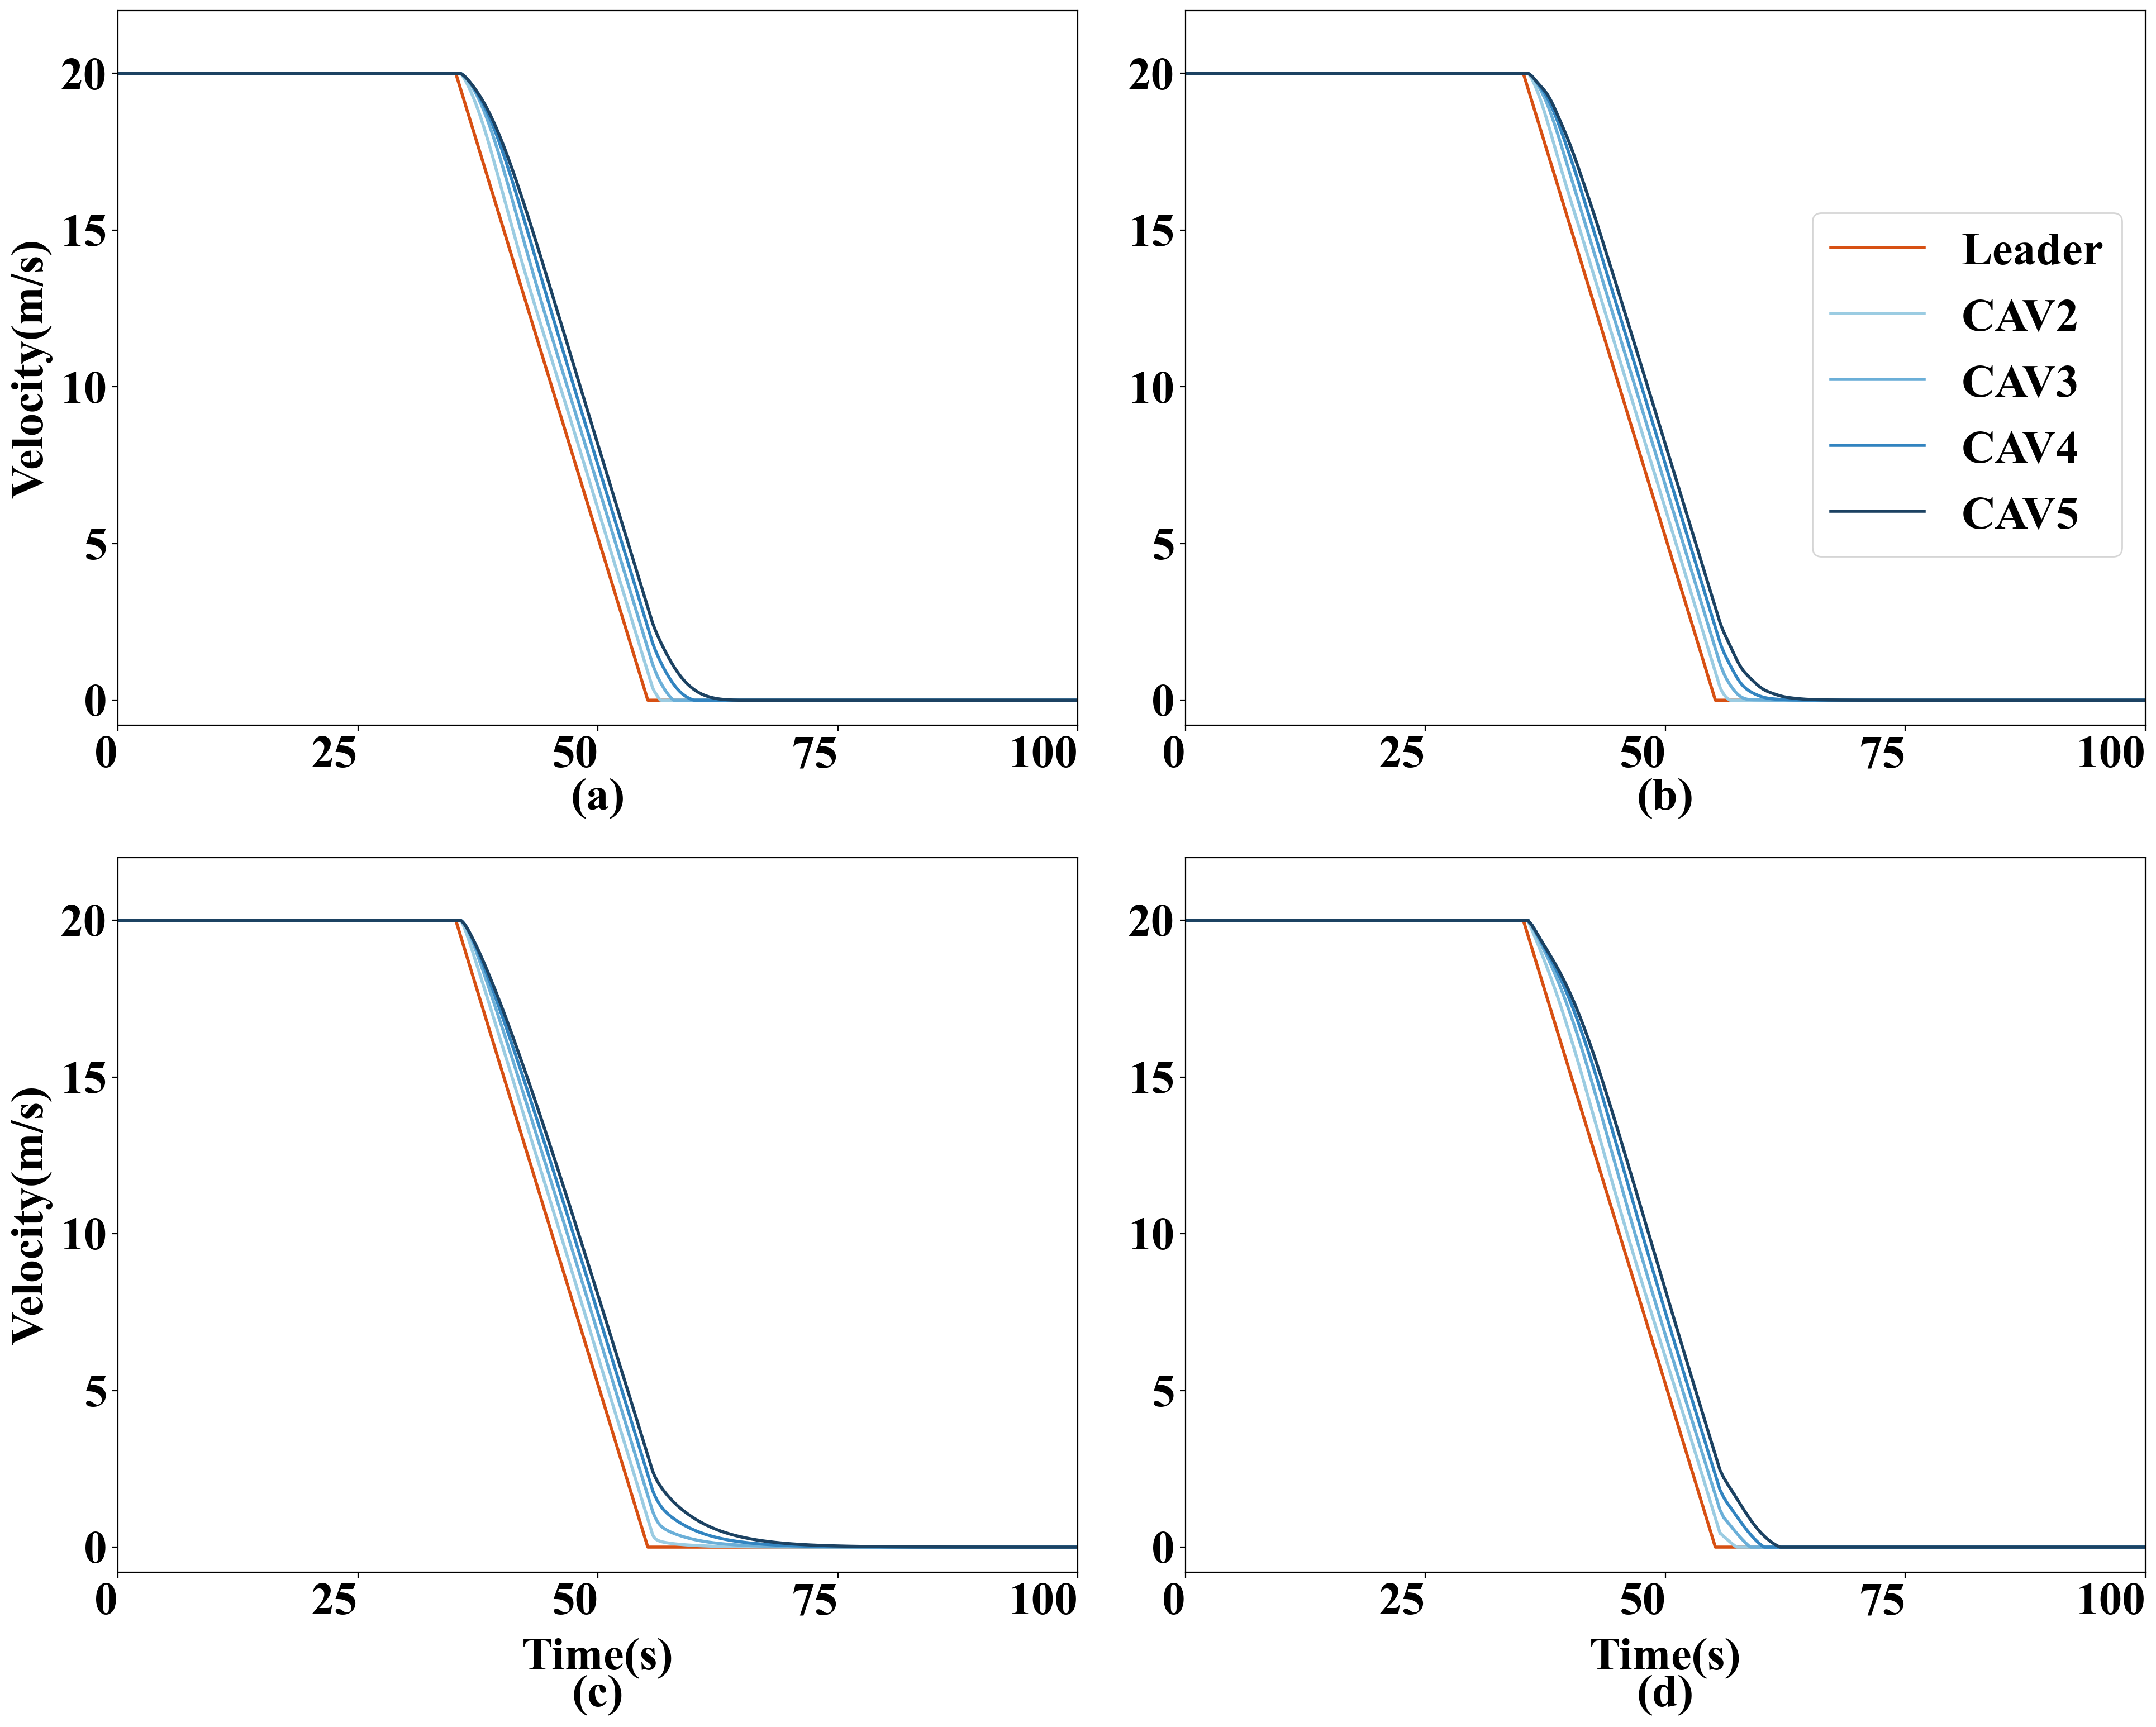
\includegraphics[width=14cm]{figs/fig7.png}
  \caption{~Tracking performance for a hard braking maneuver for each IFT under investigation: (a) PF; (b) PLF; (c) BD; (d) BDL.}
  \label{fig7}
\end{figure}


\begin{figure}

  \centering
  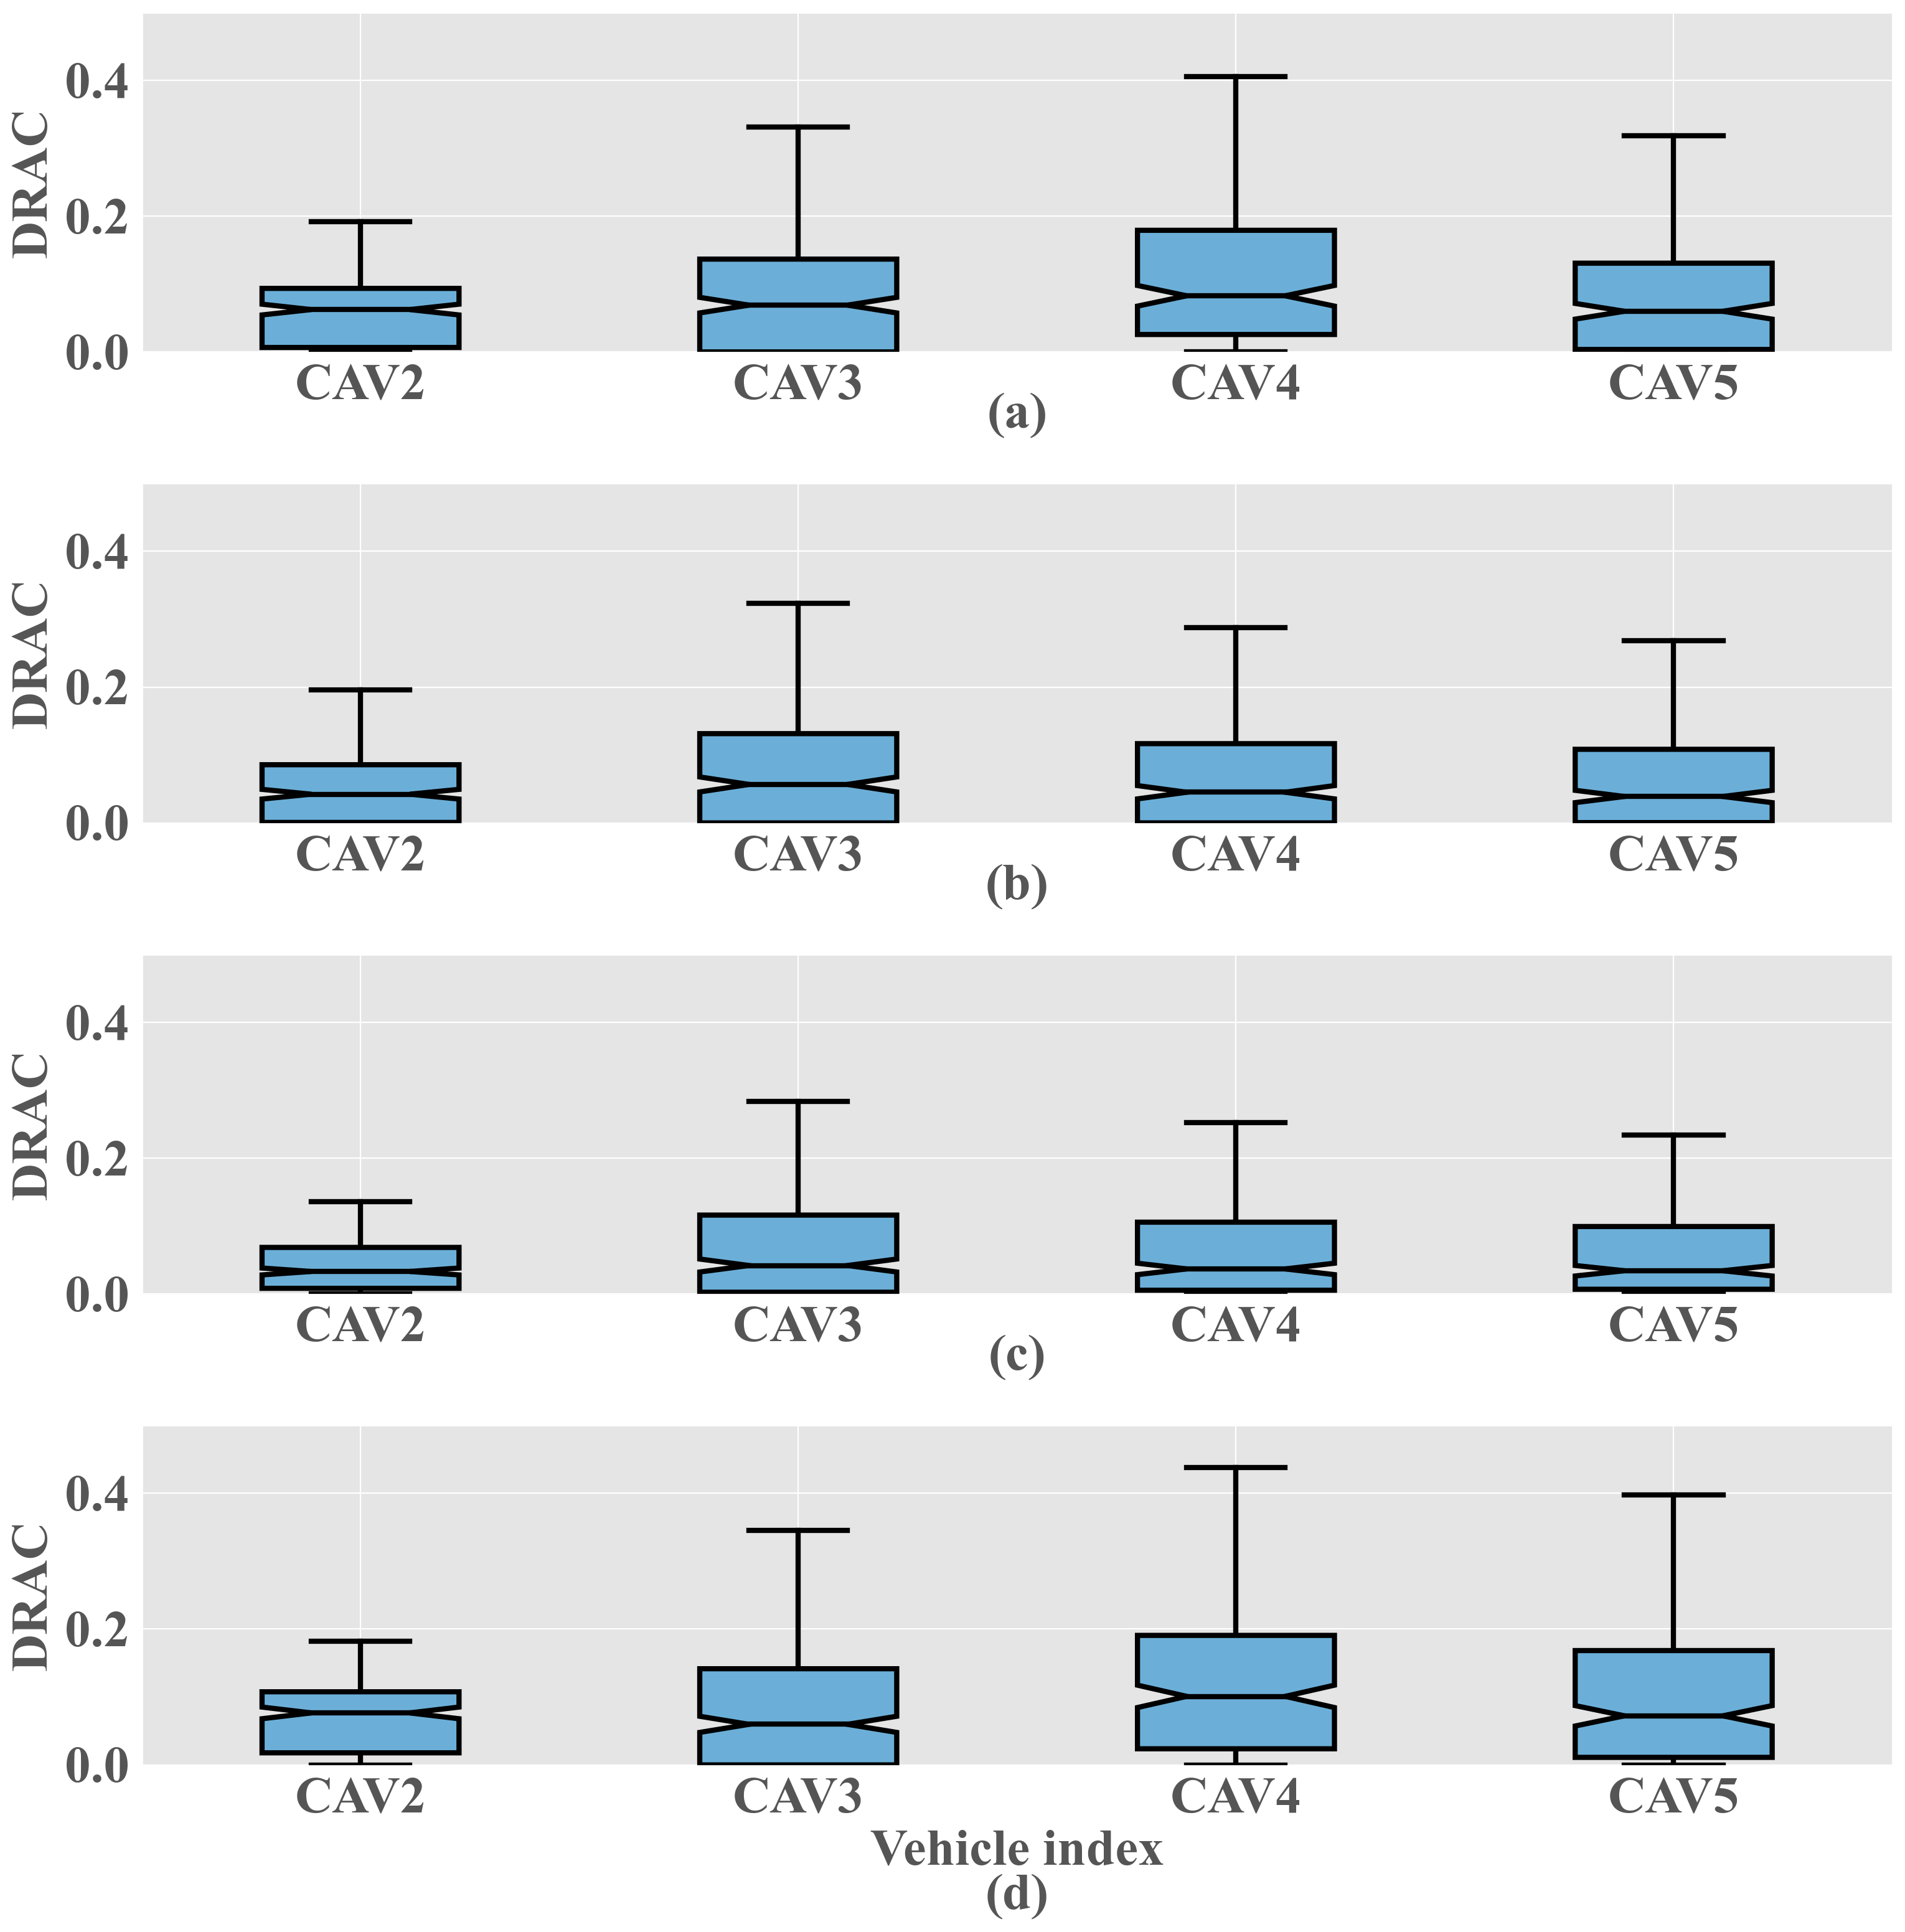
\includegraphics[width=14cm]{figs/fig8.png}
  \caption{~The DRAC boxplots for each CAV of each IFT under investigation: (a) PF; (b) PLF; (c) BD; (d) BDL.}
  \label{fig8}
\end{figure}
A phenomenon can be observed from Fig.~\ref{fig8} by comparing the boxes that the median DRAC of all CAVs under the leader-based IFTs is significantly lower than that under PF and BD at around 0.015. Therefore, we can conclude that the leader-based IFTs can maintain better safety conditions relative to PF and BD. Besides another conclusion can be obtained by comparing different CAVs under the same IFT. That is, although the control parameters are the same, the index in the platoon affects the safety conditions unless leader-based IFTs are adopted.

\subsection{Numerical analyses of the heterogeneous CAV platoon}
In this subsection, the parameters in Table~\ref{table1} are still adopted for both network and traffic simulation. The difference is the control parameters for each CAV are set heterogeneously as in Table~\ref{table2} to simulate a heterogeneous CAV platoon. It is worth mentioning that the heterogeneous control parameters chosen here still exist matrixes $P,S,Q,R,$ and $X$ satisfy the Theorem~\ref{theorem6} which can be found in Appendix B.

\begin{table}
  \centering
  \setlength{\abovecaptionskip}{0pt}
  \setlength{\belowcaptionskip}{10pt}%设置标题与表格的距离
  \begin{threeparttable}[b]

    \caption{~Control parameters for heterogeneous CAV platoon.}
    \label{table2}
    {\begin{tabular}{lc} \toprule
        Parameters                             & Value                                           \\ \midrule
        Desired time headway $h_i$             & $
        \left\{ \begin{gathered}
            0.8\quad for\quad i = 2; \hfill \\
            0.6\quad for\quad i = 3; \hfill \\
            0.7\quad for\quad i = 4; \hfill \\
            0.6\quad for\quad i = 5. \hfill \\
          \end{gathered}  \right. $                                            \\
        Feedback control gain vector $ {k_i} $ & $ \left\{ \begin{gathered}
            {[0.2,0.4,0.2]^T}\quad for\quad i = 2; \hfill \\
            {[0.3,0.3,0.2]^T}\quad for\quad i = 3; \hfill \\
            {[0.3,0.4,0.3]^T}\quad for\quad i = 4; \hfill \\
            {[0.3,0.4,0.2]^T}\quad for\quad i = 5. \hfill \\
          \end{gathered}  \right. $ \\
        \bottomrule
      \end{tabular}}
  \end{threeparttable}
\end{table}

As in Section~\ref{Section 5.2}, the two representative leader maneuvers defined in Section~\ref{Section 5.1} are employed to investigate the tracking performance of different IFTs under the heterogeneous CAV platoon. The tracking performance of the heterogeneous CAV platoon under the trapezoidal signal is presented in Fig.~\ref{fig9} and the case under the oscillatory signal is presented in Fig.~\ref{fig10}.


\begin{figure}

  \centering
  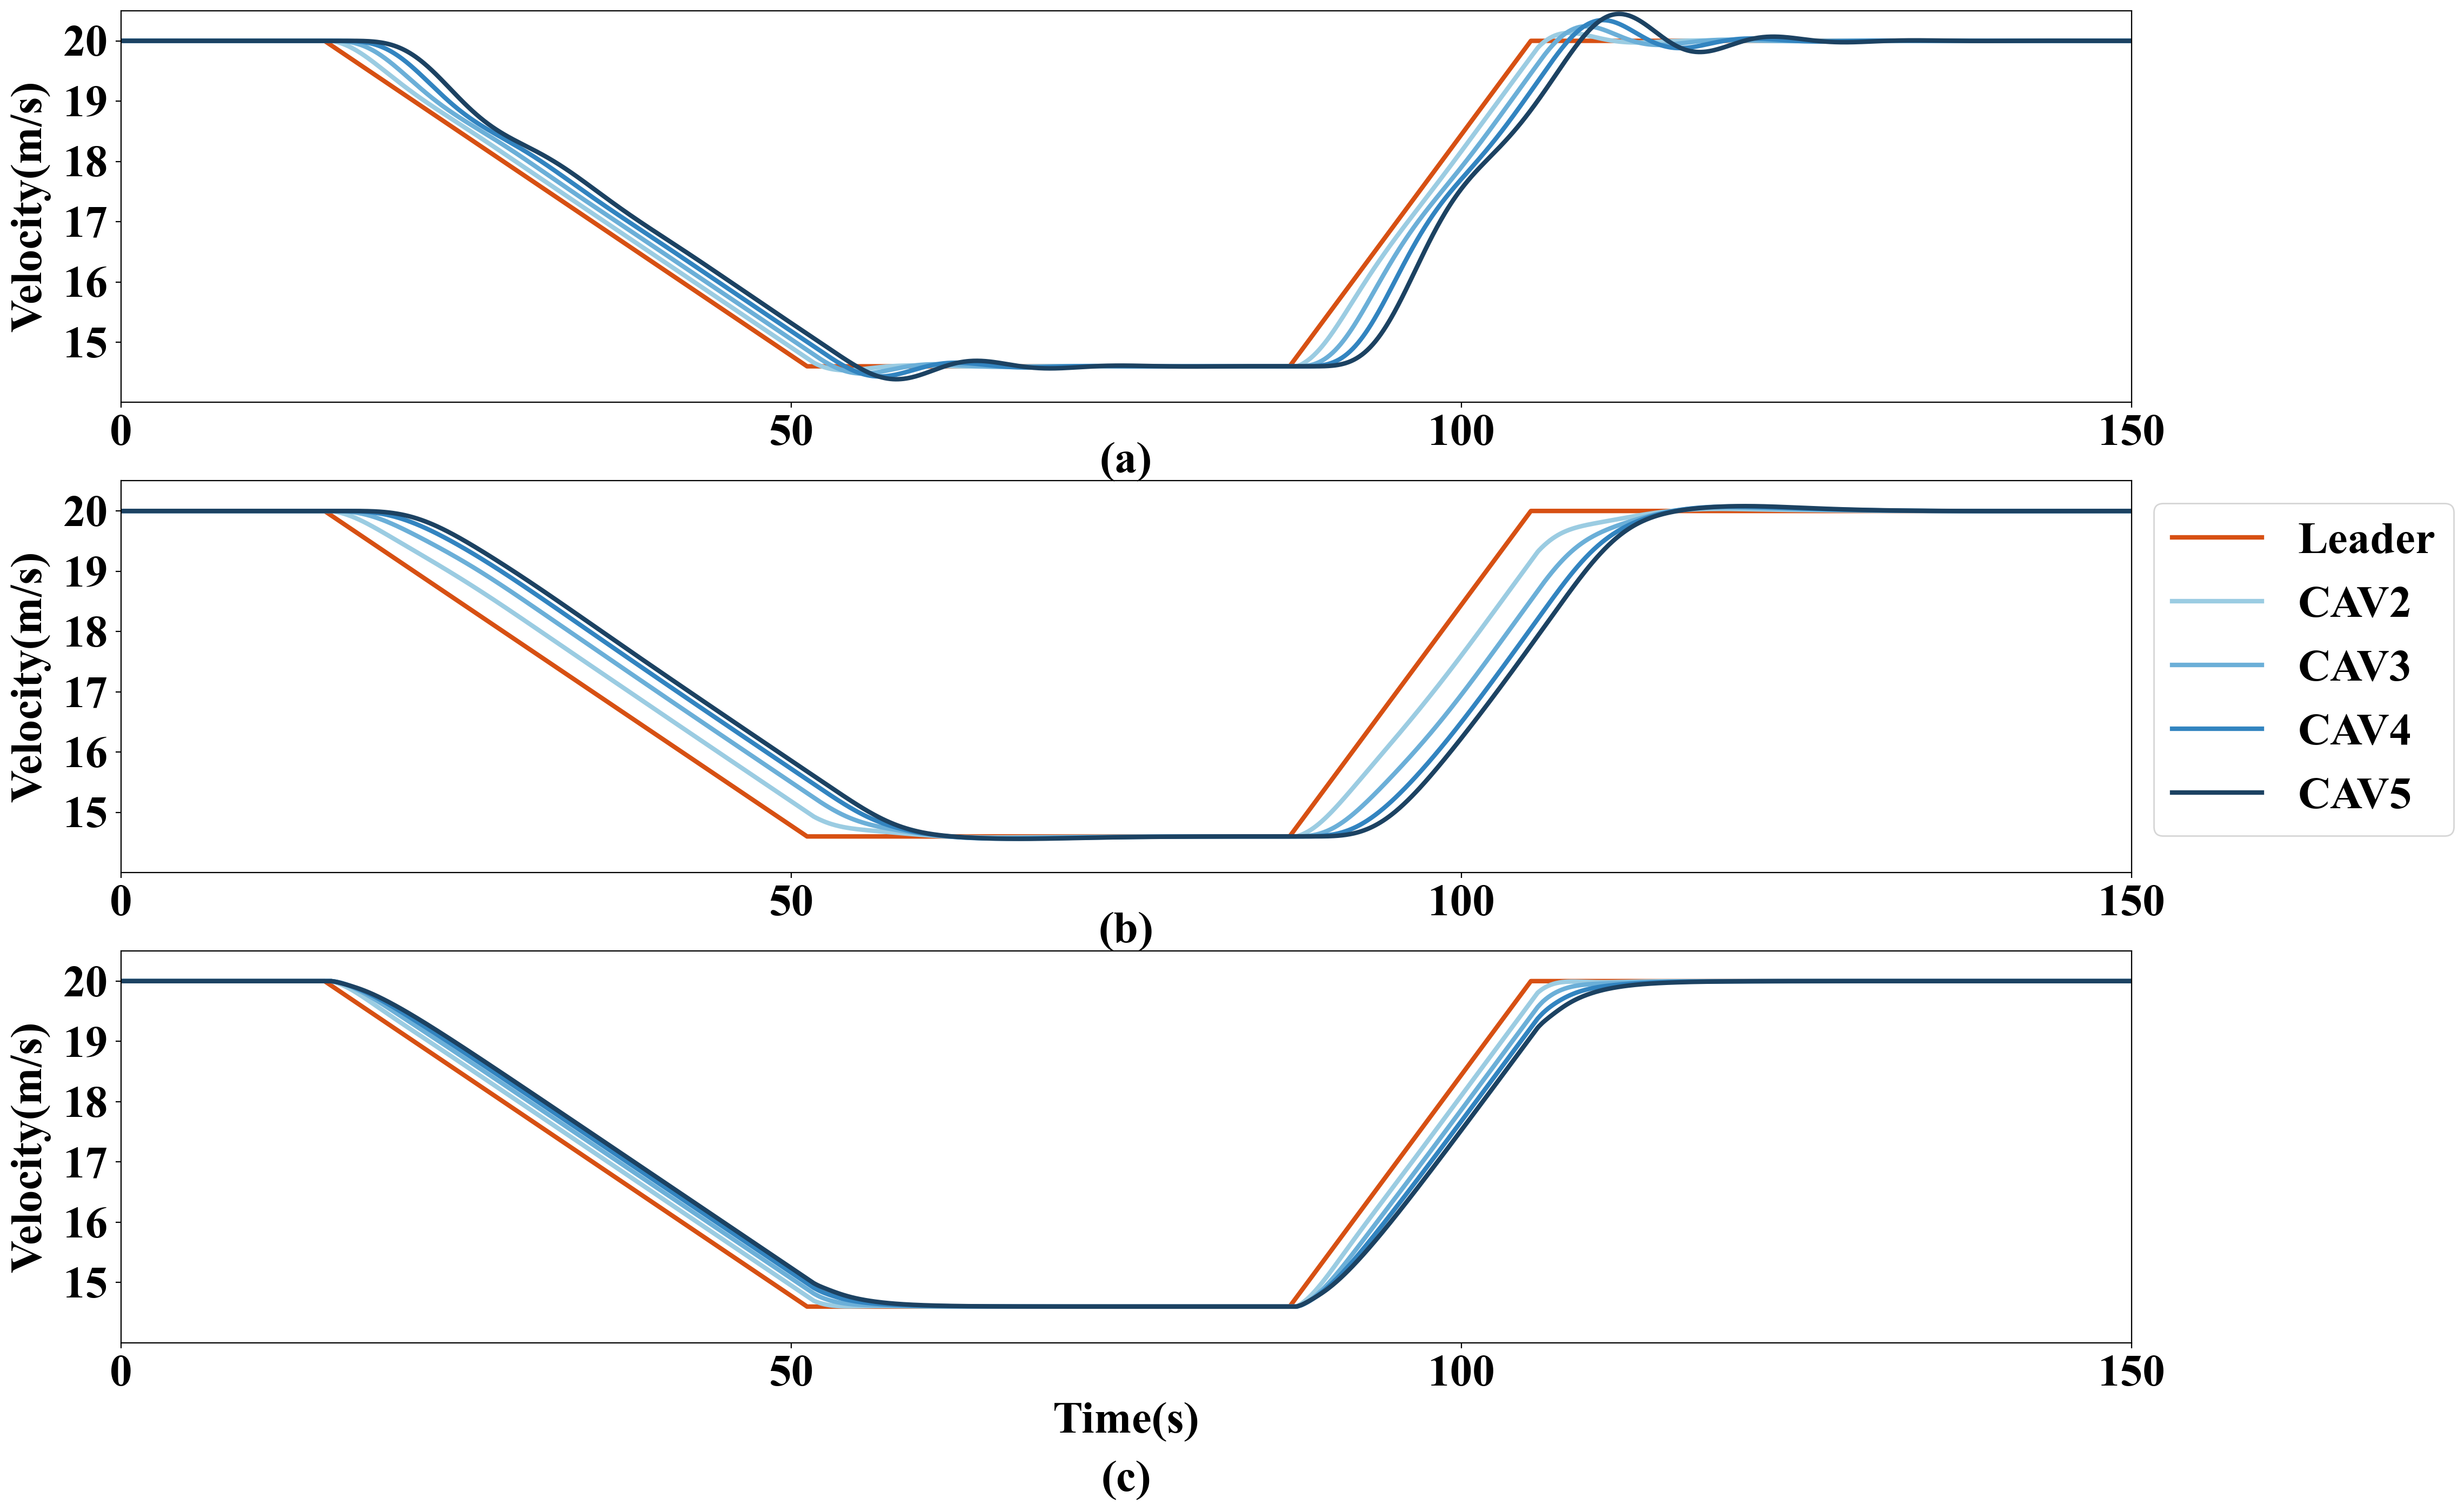
\includegraphics[width=14cm]{figs/fig9.png}
  \caption{~Tracking performance of the heterogeneous CAV platoon for the Trapezoidal signal in Fig. 3(a,b) under the four IFTs: (a), (b), (c), and (d) present tracking results under PF, including the velocity, tracking error of position, tracking error of velocity, and tracking error of acceleration, respectively; (e), (f), (g), and (h) show the case under PLF; (i), (j), (k), and (l) denote the case under BD; (m), (n), (o), and (p) show the case under BDL.}
  \label{fig9}
\end{figure}


\begin{figure}

  \centering
  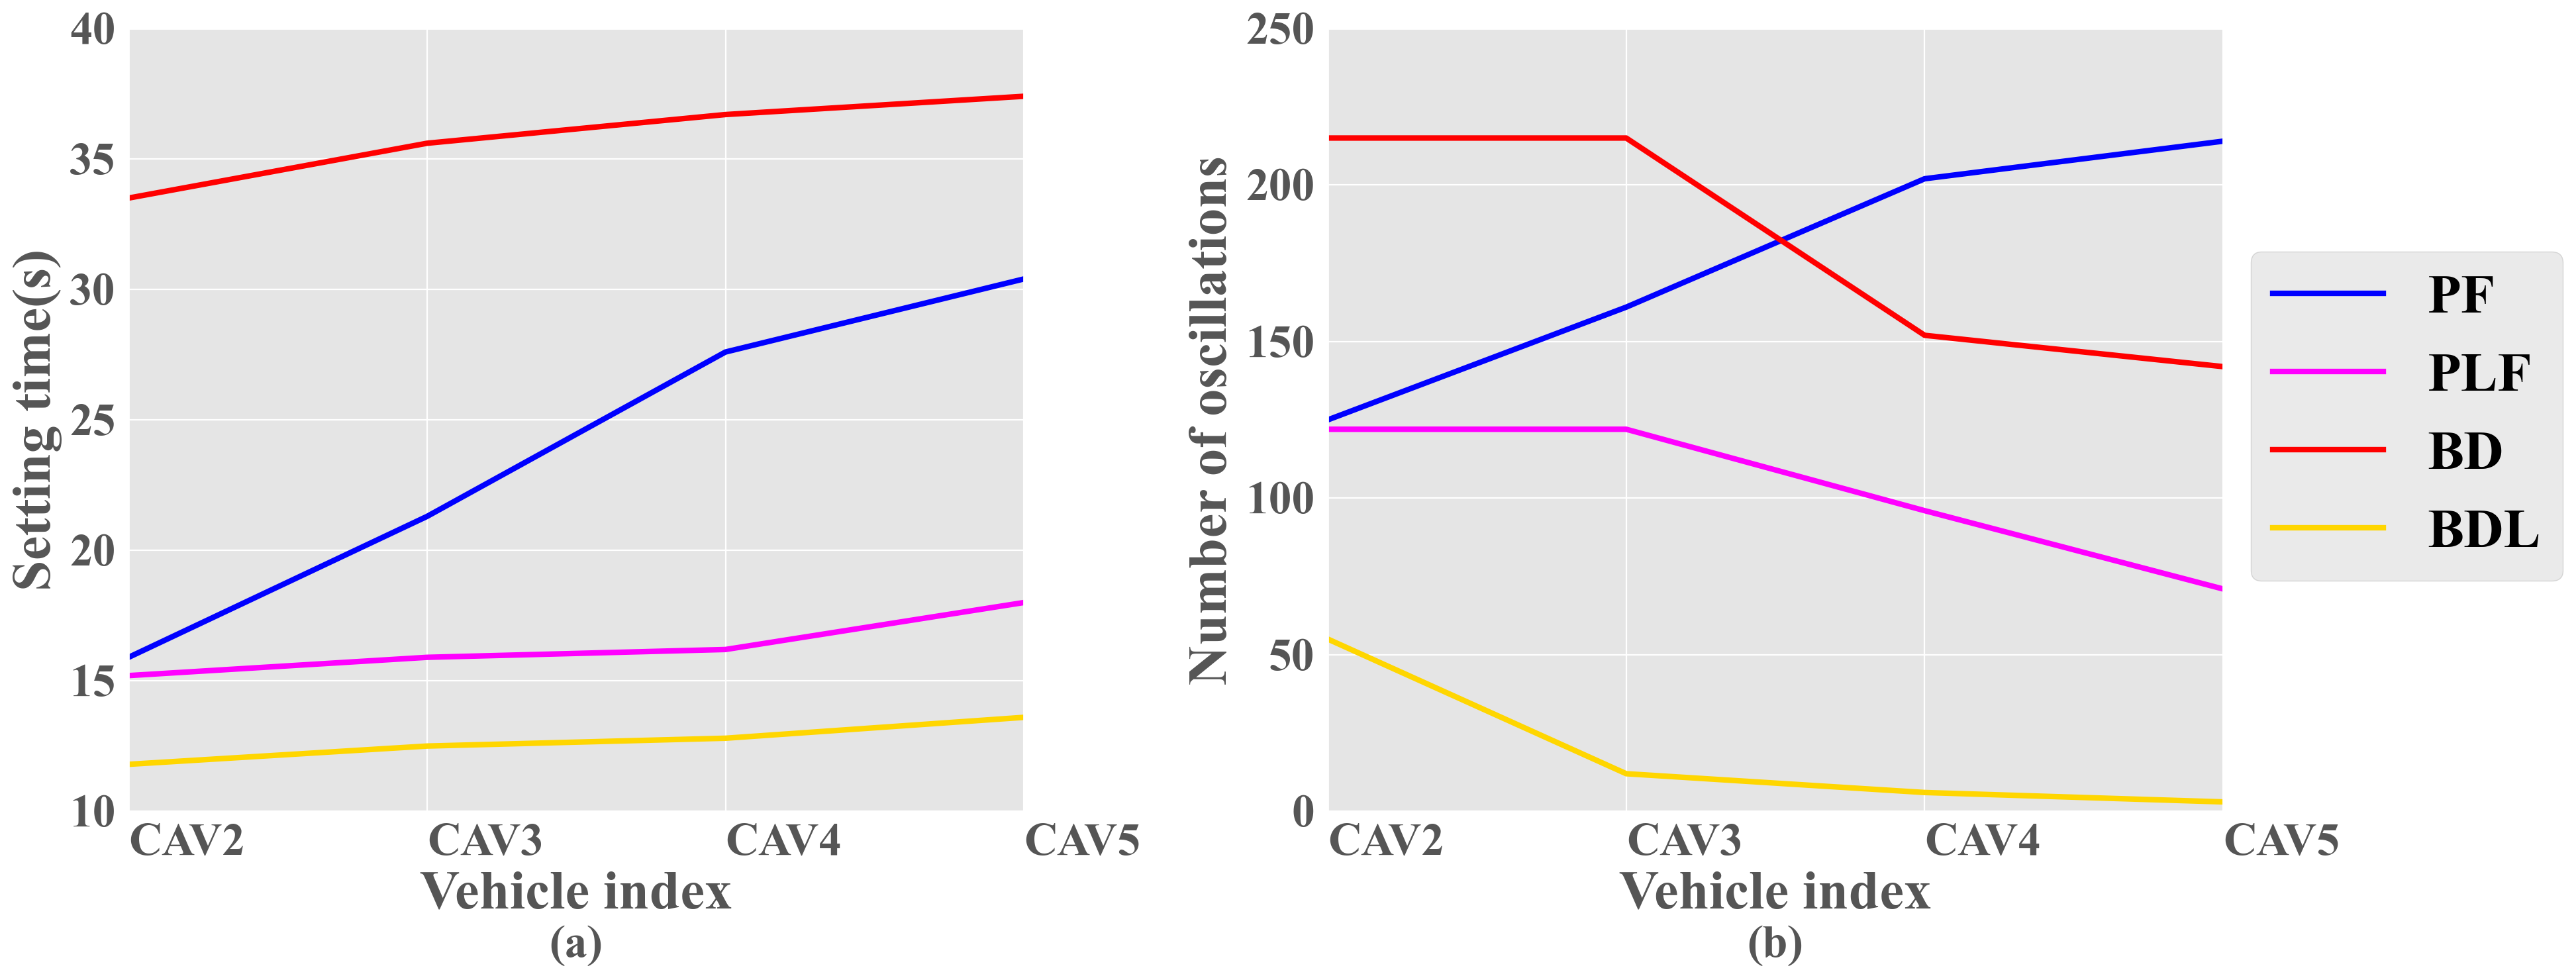
\includegraphics[width=14cm]{figs/fig10.png}
  \caption{~Tracking performance of the heterogeneous CAV platoon for the Oscillation signal in Fig. 3(c,d) under the four IFTs: (a), (b), (c), and (d) present tracking results under PF, including the velocity, tracking error of position, tracking error of velocity, and tracking error of acceleration, respectively; (e), (f), (g), and (h) show the case under PLF; (i), (j), (k), and (l) denote the case under BD; (m), (n), (o), and (p) show the case under BDL.}
  \label{fig10}
\end{figure}

A similar phenomenon can be observed that the transient response arising from tracking Leader motion gradually decreases over time thanks to stability. The difference is that the different control parameters selected for each CAV resulted in different response results. Moreover, by setting a larger desired time headway, the tracking performance can be significantly improved with smaller tracking errors. Furthermore, by comparing CAV3 and CAV5 which apply the same desired time headway and different feedback control gain, it can be found that CAV3 can significantly decrease the tracking error from CAV2 while CAV5 cannot. Therefore, it can be concluded that the effect of different feedback control gain on tracking performance is significant.



\section{Conclusion and future work}
\label{Section 6}

In this paper, a generic supermatrix modeling approach for the CAV platoon considering time-varying communication delay is proposed. This generic modeling approach consists of applying graph theory to describe the communication relationships within a CAV platoon generally defined by IFT and modeling the linear time-invariant state time-varying delay system corresponding to the the CAV platoon that employs a CTH control strategy with the help of supermatrices. Furthermore, based on the properties of the linear time-invariant state time-varying delay system, a novel stability condition of the generic CAV platoon is derived by applying Wirtinger-Based Integral Inequality and Lyapunov-Krasovskii Stability Theorem. Furthermore, extensive numerical analyses are conducted to comprehensively evaluate the tracking performance and safety conditions of four typical IFTs and thus provide guidance for the selection of IFTs. At last, a comparison on the tracking performance between the homogeneous CAV platoon and the heterogeneous CAV platoon sheds some light on the selection of control parameters.

The following conclusions can be drawn through numerical analysis:
\begin{enumerate}
  \item All CAVs under each IFT are capable of tracking error and returning to equilibrium with assurance so that the stability conditions are satisfied.
  \item From the control objectives of accuracy and speed, the application of Leader-based IFTs can enable smoother tracking performance and avoid overshooting compared to other IFTs. Besides, safer driving can be achieved by communicating with the Leader.
  \item As for the difference between uni- and bi-directional communication, bi-directional communication can effectively balance the tracking performance among the CAV platoon even when the CAV platoon is long, while uni-directional communication delivers deteriorating tracking performance as the CAV platoon length increases.
  \item The effect of different feedback control gains on tracking performance is significant.
\end{enumerate}

However, we acknowledge that the vehicle behavior in the simulation is only a simplification of reality, and further field experiments are needed for providing a more accurate analysis of the tracking performance. Likewise, the time-varying delay function applied in this paper is an assumed Bessel function satisfying the condition that both the delay and its derivative are bounded, which does not fit the actual time-varying delay perfectly. Therefore, corresponding field experiments should also be conducted to provide insights into the time-varying relationship of communication delays. Furthermore, the control parameter scheme that yields the optimal tracking performance should be further investigated through theoretical research and field experiments. Future research should also be directed toward designing novel control strategies to enable smoother and safer tracking performance.


\appendix


\section*{Appendix A.~Feedback control for linearization}
\label{AppendixA}
In this appendix, we provide the linearization of the longitudinal vehicle dynamic in Equation (\ref{eq1}). The functions of the lumped uncertain resistance forces, including $f_i^g(t)$, $f_i^w(t)$, and $f_i^r(t)$ are expressed as follows:
\begin{equation}
  \left\{\begin{array}{l}
    f_{i}^{g}(t)=m_{i} g \sin \left(\theta_{i}(t)\right)                        \\
    f_{i}^{w}(t)=\frac{1}{2} \rho C_{D} A_{F}\left(v_{i}(t)+v_{w}(t)\right)^{2} \\
    f_{i}^{r}(t)=\mu_{R} m_{i} g \cos \left(\theta_{i}(t)\right)
  \end{array}\right.
  \label{eqapp5}
\end{equation}
where $g=9.81m/s^2$ denotes the acceleration of gravity; $\theta_i(t)$ is the inclination angle of the road; $\rho$ denotes the air density; $C_D$ is the aerodynamic drag coefficient; $A_F$ represents the maximal cross-sectional/frontal area of the vehicle; $v_w(t)$ denotes the uncertain headwind speed; $\mu_R$ is the coefficient of rolling resistance.

The desired engine dynamic is modeled as follows:
\begin{equation}
  (\tau_is+1)F_i^e=U_i
  \label{eqapp6}
\end{equation}

Adopting the inverse Laplace transformation on Equation (\ref{eqapp6}) arrives at:
\begin{equation}
  \dot{f_i^e}\left(t\right)=\frac{u_i(t)}{\tau_i}-\frac{f_i^e\left(t\right)}{\tau_i}
  \label{eqapp7}
\end{equation}

Substituting Equation (\ref{eq1}) into Equation (\ref{eqapp7}) and differentiating both sides of Equation (\ref{eqapp7}) with respect to time, we get:
\begin{equation}
  \begin{aligned}
    \dot{a}_{l}(t) & =\frac{\dot{f}_{l}^{e}(t)}{m_{i}}-\frac{\dot{f}_{l}^{g}(t)}{m_{i}}-\frac{f_{l}^{i \omega}(t)}{m_{i}}-\frac{\dot{f}_{l}^{r}(t)}{m_{i}}                                                                                         \\
                   & =               \frac{u_{i}(t)}{m_{i} \tau_{i}}                                                                                                                                                                               \\
                   & -               \frac{a_{i}(t)+\mathrm{g} \sin \left(\theta_{i}(t)\right)\left[1-\tau_{i} \mu_{R} \dot{\theta}_{l}(t)\right]+\mathrm{g} \cos \left(\theta_{i}(t)\right)\left[1+\tau_{i} \dot{\theta}_{l}(t)\right]}{\tau_{i}} \\
                   & -               \frac{\frac{1}{2} \rho C_{D} A_{F}\left(v_{i}(t)+v_{w}(t)\right)\left(\left(v_{i}(t)+v_{w}(t)\right)+2 \tau_{i}\left(a_{i}(t)+\dot{v}_{w}(t)\right)\right)}{\tau_{i}}
  \end{aligned}
  \label{eqapp8}
\end{equation}

Thus, the nonlinear state feedback chosen for linearizing can be defined by:
\begin{equation}
  \begin{aligned}
    u_i^\ast\left(t\right)= & m_iu_i\left(t\right)+g\sin{\left(\theta_i\left(t\right)\right)}\left[1-\tau_i\mu_R\dot{\theta_i}\left(t\right)\right]+g\cos{\left(\theta_i\left(t\right)\right)}\left[1+\tau_i\dot{\theta_i}\left(t\right)\right]\ \\
                            & +\frac{1}{2}\rho C_DA_F\left(v_i\left(t\right)+v_w\left(t\right)\right)\left(\left(v_i\left(t\right)+v_w\left(t\right)\right)+2\tau_i(a_i\left(t\right)+\dot{v_w}\left(t\right))\right)
  \end{aligned}
  \label{eqapp9}
\end{equation}

Under the new feedback control input, the Equation (\ref{eq1}) can be rewritten as:
\begin{equation}
  \tau_i\dot{a_i}\left(t\right)+a_i\left(t\right)=u_i(t)
  \label{eqapp10}
\end{equation}





\section*{Appendix B.~Attachments uploaded to GitHub}
\label{AppendixB}
The uploaded code of this paper contains the model formulation of Theorem~\ref{theorem3} and the construction of LMIs for Theorem~\ref{theorem6}. In addition, the matrices corresponding to the two sets of control parameters for the homogeneous and heterogeneous CAV platoon selected in Section~\ref{Section 5}, which are compatible with Theorem~\ref{theorem6}, have also been uploaded. The URL of the uploaded file repository is:
https://github.com/ruantiancheng/code-of-paperGeneral-heterogeneous-CAV-platoon-considering-the-time-varying-communication-delay.
% \afterpage{\clearpage}

\printcredits

\section*{Acknowledgment}

This research was sponsored by the National Science Foundation of China (No. 51878161 and No.52072067), Postgraduate Research \& Practice Innovation Program of Jiangsu Province (KYCX22\_0266), Natural Science Foundation of Jiangsu Province (No. BK20210249) and Jiangsu Planned Projects for Postdoctoral Research Funds (No. SBK2021041144).

%% Loading bibliography style file
% \bibliographystyle{model1-num-names}
\bibliographystyle{cas-model2-names}

% Loading bibliography database
\bibliography{cas-refs}


%\vskip3pt

\end{document}

